\documentclass[11pt]{article}

\usepackage[margin=1in]{geometry}
\usepackage{amsmath,amssymb,amsfonts,bm}
\usepackage{graphicx}
\usepackage{xcolor}
\usepackage{float}
\usepackage{listings}
\usepackage{enumitem}
\usepackage{booktabs}
\usepackage{hyperref}
\usepackage{xurl}
\usepackage{fancyhdr}

% ---------- URL and Hyperlink setup ----------
\Urlmuskip=0mu plus 1mu
\hypersetup{
	breaklinks=true,
	colorlinks=true,
	linkcolor=blue,
	urlcolor=blue
}

% ---------- MATLAB code style ----------
\lstdefinestyle{matlabstyle}{
	language=Matlab,
	basicstyle=\ttfamily\small,
	numbers=left,
	numberstyle=\tiny,
	stepnumber=1,
	numbersep=8pt,
	frame=single,
	columns=fullflexible,
	keepspaces=true,
	showstringspaces=false,
	keywordstyle=\bfseries,
	commentstyle=\itshape\color{gray},
}

% ---------- Header setup ----------
\pagestyle{fancy}
\fancyhf{}
\fancyhead[L]{\today}
\fancyhead[C]{ECE 533: Homework \#1}
\fancyhead[R]{Scott Nguyen}
\renewcommand{\headrulewidth}{0.4pt}
\fancyfoot[C]{\thepage}

\begin{document}
	
	\noindent
	\textbf{Homework 1: An Introduction to Image Processing Using Python}
	
	For this homework, refer to the tutorials given in 
	\href{https://github.com/pattichis/AIML}{my AIML GitHub repo}.
	
	Unless otherwise stated, you can assume that the homework refers to 8-bit grayscale images (e.g., problem 1).
	
	For full credit, you must submit:
	\begin{itemize}
		\item A. Screenshots of images involved.
		\item B. Python code. PDFs are fine.
		\item C. Discussion is always required for all parts. Often, a single sentence is NOT enough. You need to comment on what your images represent.
	\end{itemize}
	
	\vspace{1em}
	
	% ---------------- Problem 1 ----------------
	\noindent
	\textbf{Problem 1. Basic Image Representations (20 points)}
	
	Use the 
	\href{http://ivpcl.unm.edu/ivpclpages/Research/aolme/app/interactive-img-v2.html}{interactive image editor}
	to generate:
	
	\begin{enumerate}[label=\textbf{\Alph*.}, leftmargin=1.2cm]
		\item A binary image.
		\item A greyscale image.
		\item A color image.
	\end{enumerate}
	
	\vspace{1em}
	\noindent\textbf{Solution.}
	
	\begin{enumerate}[label=\textbf{(\alph*)}, leftmargin=1.2cm]
		
		% ---------------- (a) ----------------
		\item \textbf{Binary Image}
		
		\begin{figure}[H]
			\centering
			
\includegraphics[width=0.35\textwidth]{plots/binary.png}
			\caption{Binary checkerboard image generated in Python.}
		\end{figure}
		
		\textbf{Discussion:}  
		This is a binary image because each pixel is restricted to only two intensity values, 0 (black) and 1 (white).  
		The checkerboard arrangement creates sharp transitions between neighboring pixels, producing very high contrast and clearly defined edges. Binary images are commonly used in segmentation, thresholding, and logical masking operations where only two classes are required.
		
		
		\vspace{1em}
		
		% ---------------- (b) ----------------
		\item \textbf{Greyscale Image}
		
		\begin{figure}[H]
			\centering
			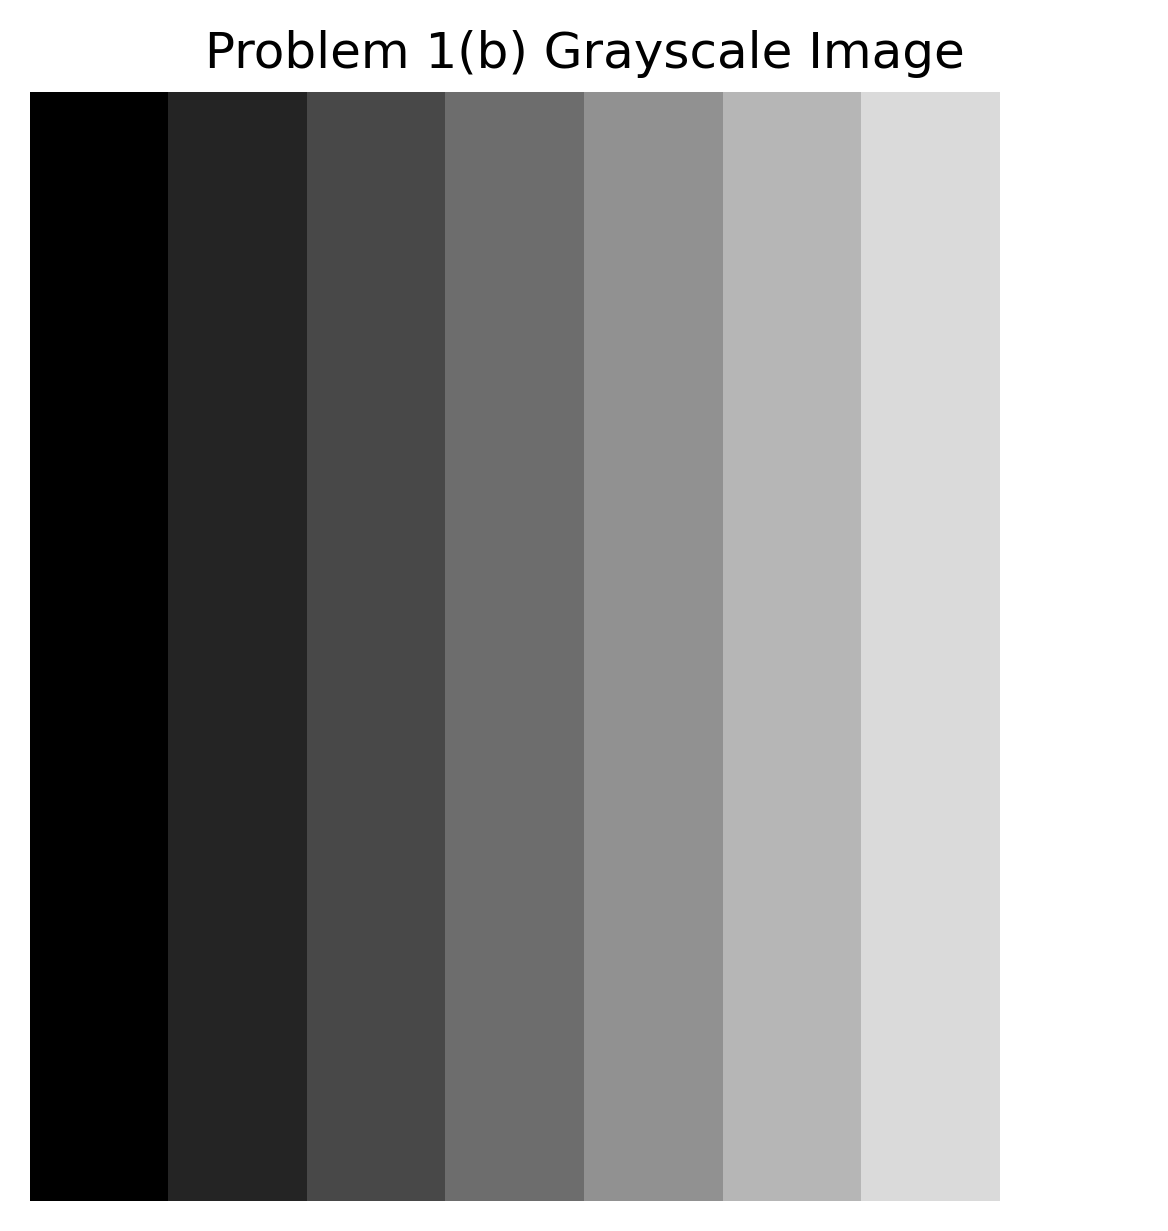
\includegraphics[width=0.35\textwidth]{plots/grayscale.png}
			\caption{Greyscale gradient image generated in Python.}
		\end{figure}
		
		\textbf{Discussion:}  
		This greyscale image uses 8-bit intensity values ranging from 0 to 255.  
		The gradual horizontal transition from dark to bright demonstrates how greyscale images represent smooth variations in brightness and shading. Compared to binary images, greyscale images preserve more detail and allow more realistic representation of continuous tones.
		
		
		\vspace{1em}
		
		% ---------------- (c) ----------------
		\item \textbf{Color Image}
		
		\begin{figure}[H]
			\centering
			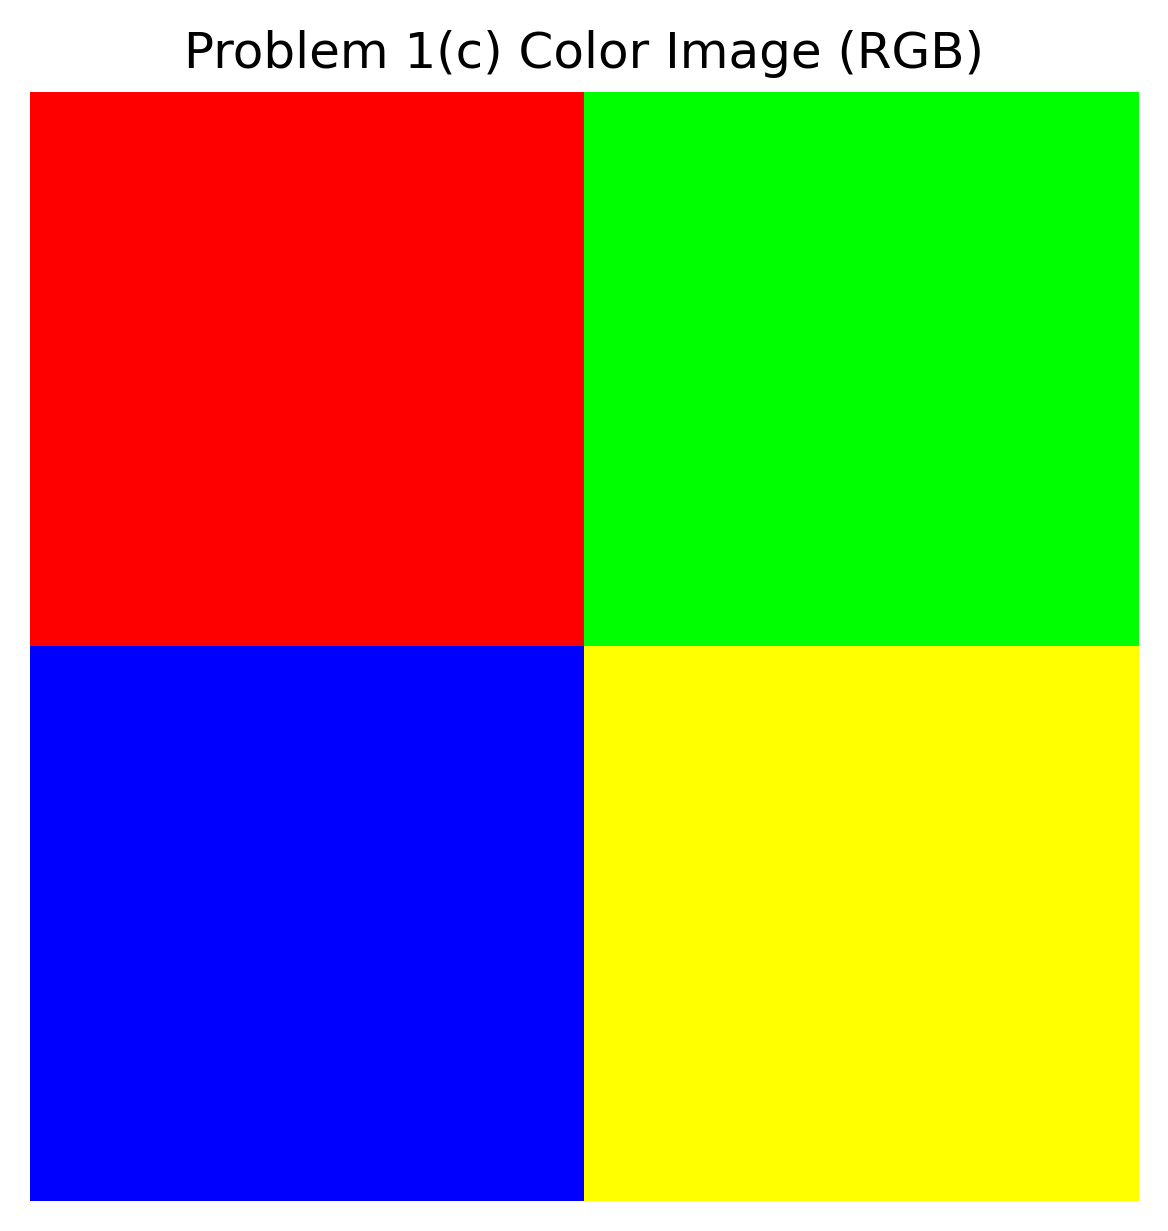
\includegraphics[width=0.35\textwidth]{plots/color.png}
			\caption{RGB color image generated in Python.}
		\end{figure}
		
		\textbf{Discussion:}  
		This image is a color image represented using three channels: red, green, and blue (RGB).  
		Each pixel stores three intensity values that combine to produce a wide range of colors. The different colored regions illustrate how varying the RGB components changes the perceived color. Color images provide richer visual information and better object differentiation compared to greyscale images.
		
	\end{enumerate}
	
	\newpage
	
	% ---------------- Problem 2 ----------------
	\noindent\textbf{Problem 2. Contrast of image patches (60 points, modified after discussion session)}
	
	For this problem, refer to 
	\href{https://colab.research.google.com/github/pattichis/AIML/blob/main/Session_8_Create_videos.ipynb#scrollTo=vhSh4F_an5j4}{example of using image patches}.
	
	Part E carries 40 points. The rest are evenly distributed among A to D.
	
	\begin{enumerate}[label=\textbf{\Alph*.}, leftmargin=1.2cm]
		
		\item Create an example with a minimum (non-zero) contrast for 8-bit grayscale images.
		
		\item Create an 8-bit grayscale image example with maximum contrast.
		
		\item Create an image with zero background and constant patches of 5, 10, 100, 200, and 250.
		
		\item Apply the logarithmic transformation $\log(1 + C \cdot I)$ for different values of $C$ and discuss the visibility of the different patches.
		
		\item Place the images from parts C and D side-by-side for $C=1, 5, 10, 100$. Create a visibility table with $C$ values along the rows and the patch values along the columns (5, 10, 100, 200, 250). In the table, provide a ranked score from 0 to 5 as follows:
		\begin{itemize}
			\item 0 means it is non-visible.
			\item 1 means it has the worst visibility among all values of $C$.
			\item 2 means it has the second-worst visibility among all values of $C$. Similarly for 3 and 4.
			\item 5 means it has the best visibility among all values of $C$.
		\end{itemize}
		
		Provide a very brief justification of how you chose your scores. You do not need to talk about all of them.
		
	\end{enumerate}
	
	\textbf{Note:} Against the zero-background, each patch will have unit local contrast (verify). However, when assessing them, your perception of them will vary based on their relative positions and sizes. Thus, not everyone will have the same values.
	
	\vspace{1em}
	\noindent\textbf{Solution.}
	
	\begin{enumerate}[label=\textbf{\Alph*.}, leftmargin=1.2cm]
		
		% ===================== A =====================
		\item \textbf{Minimum (non-zero) contrast example}
		
		\begin{figure}[H]
			\centering
			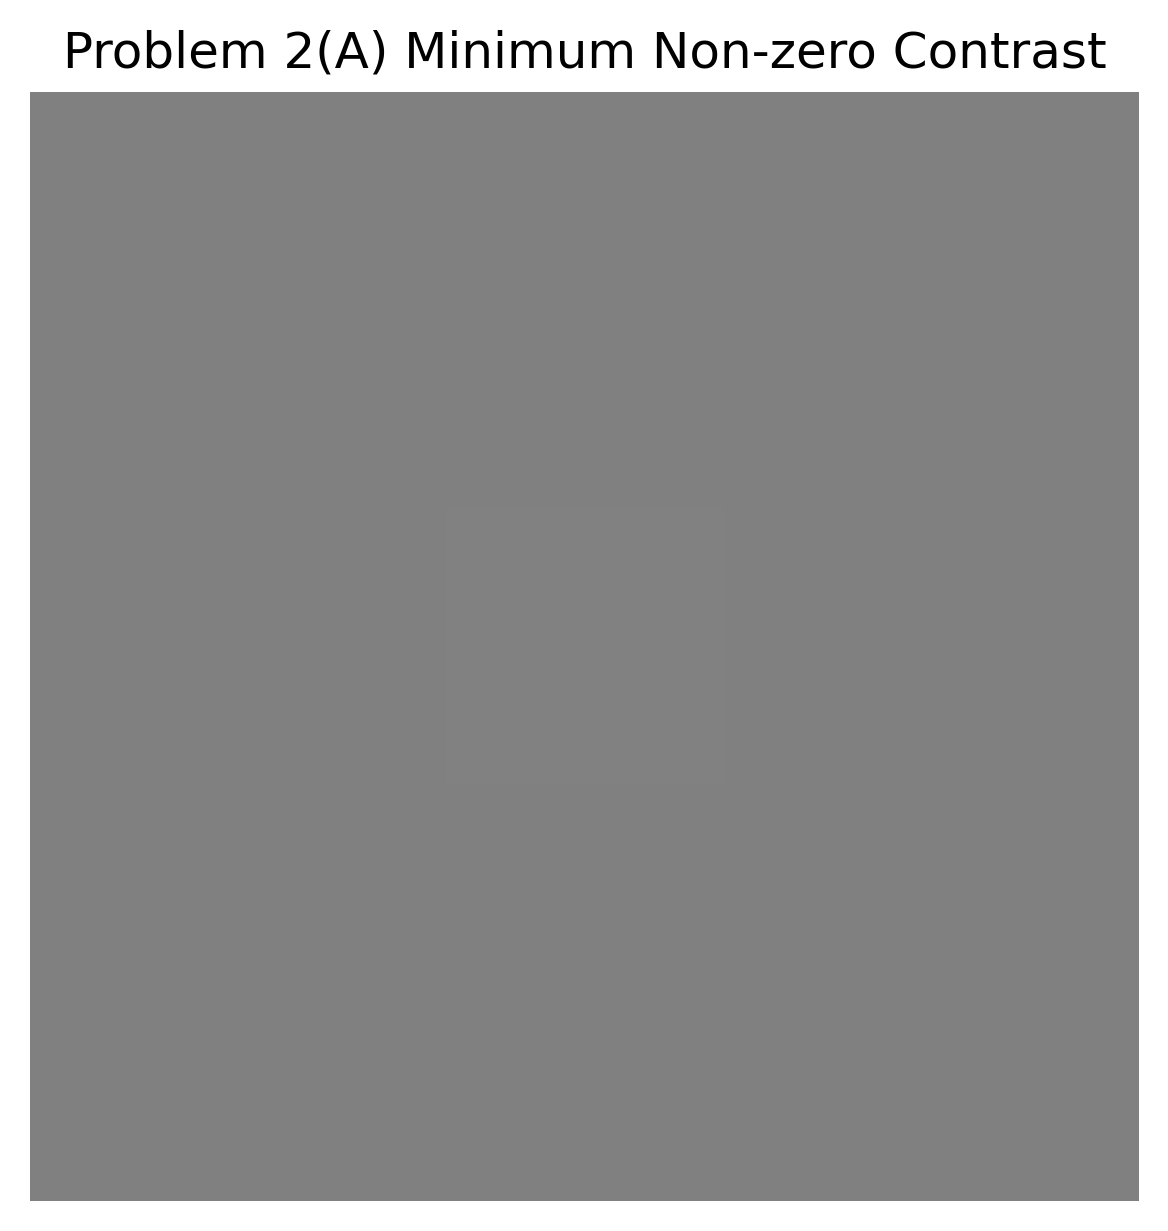
\includegraphics[width=0.6\textwidth]{plots/P2A_min_contrast.png}
			\caption{Problem 2(A): Minimum non-zero contrast (background 128, patch 129).}
		\end{figure}
		
		\textbf{Discussion:}
		This image uses an 8-bit gray background of 128 with a square patch of 129, so the intensity difference is 1 (the smallest non-zero change possible in 8-bit images). The patch is barely visible because the contrast relative to the background is extremely small. This demonstrates the practical limit of detectability when contrast is minimal.
		
		\vspace{1em}
		
		% ===================== B =====================
		\item \textbf{Maximum contrast example}
		
		\begin{figure}[H]
			\centering
			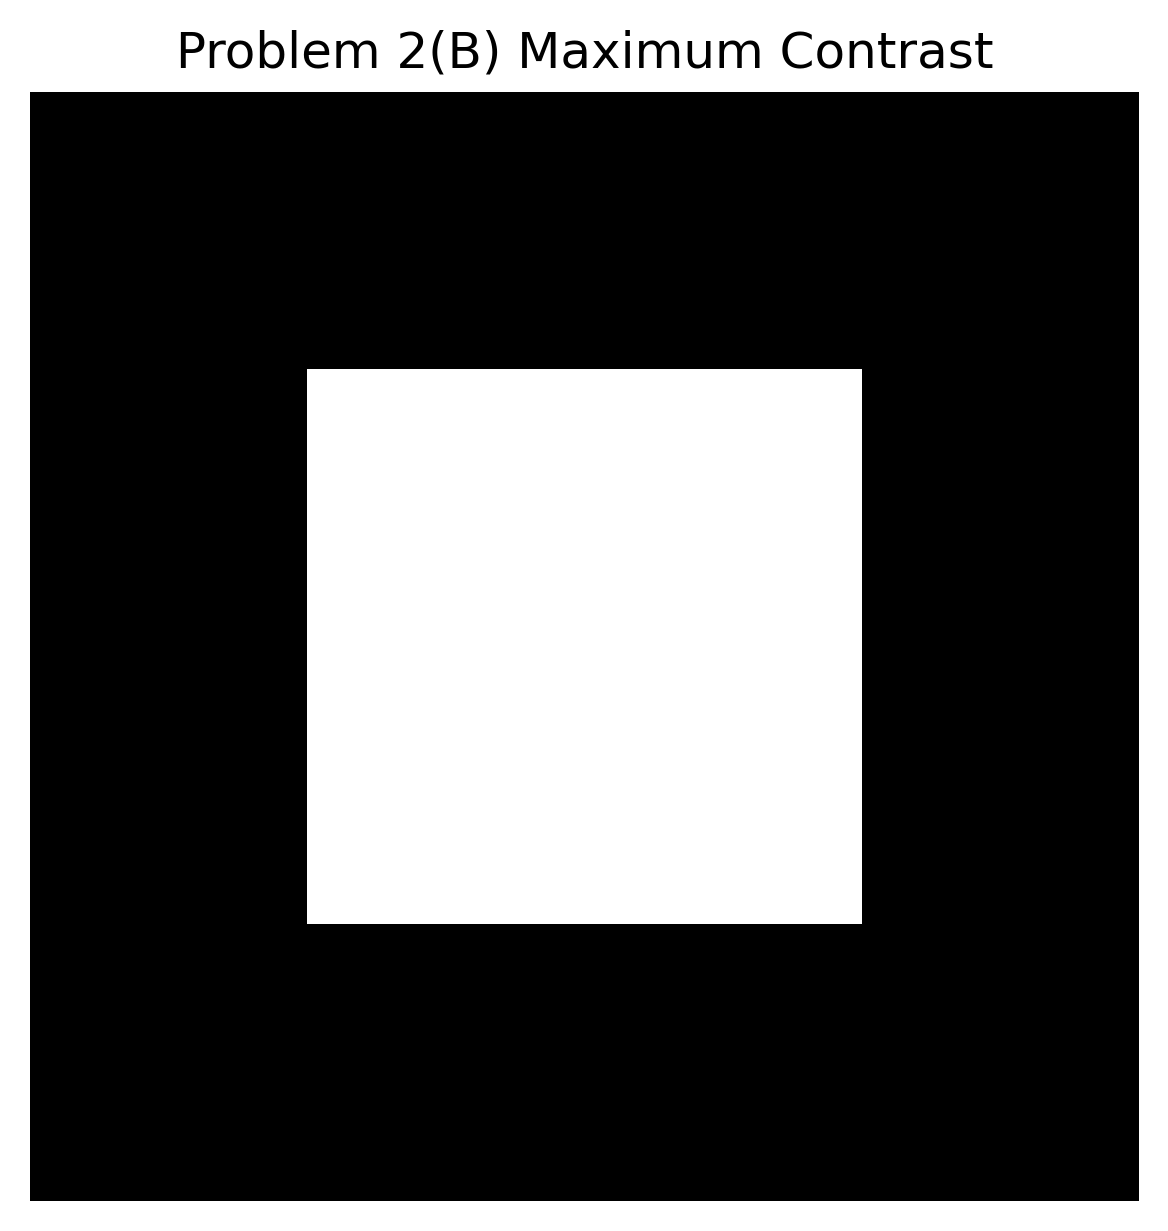
\includegraphics[width=0.6\textwidth]{plots/P2B_max_contrast.png}
			\caption{Problem 2(B): Maximum contrast (background 0, patch 255).}
		\end{figure}
		
		\textbf{Discussion:}
		This image uses a black background (0) and a white patch (255), producing the maximum possible contrast in an 8-bit image. The patch is clearly visible with sharp boundaries because the intensity difference spans the full available range.
		
		\vspace{1em}
		
		% ===================== C =====================
		\item \textbf{Zero background with constant patches}
		
		\begin{figure}[H]
			\centering
			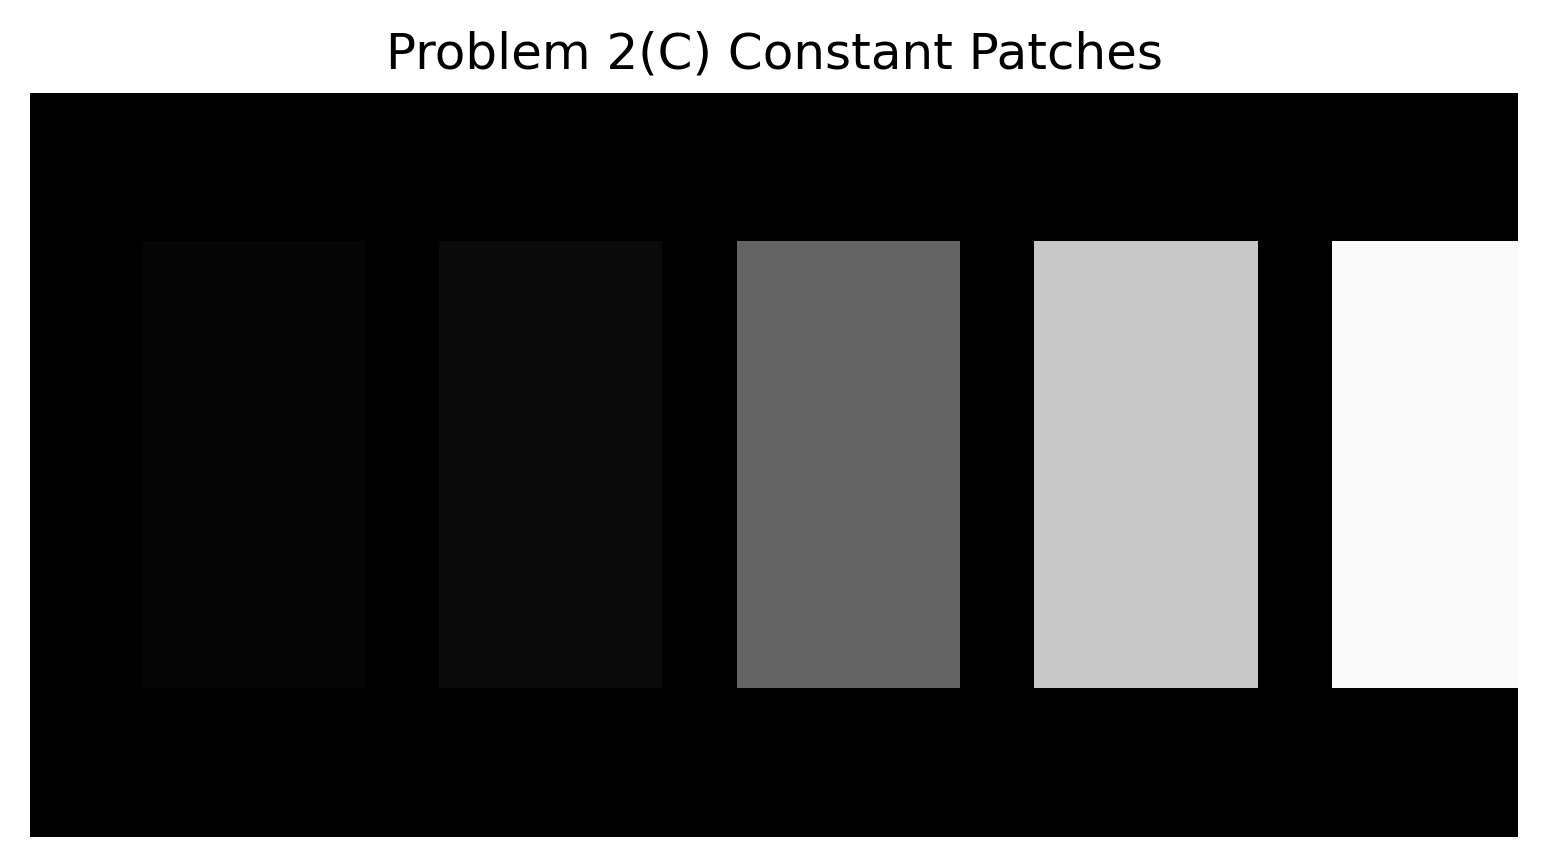
\includegraphics[width=0.85\textwidth]{plots/P2C_patches.png}
			\caption{Problem 2(C): Constant patches (5, 10, 100, 200, 250) on a zero background.}
		\end{figure}
		
		\textbf{Discussion:}
		This image contains five constant-intensity patches on a zero (black) background with values 5, 10, 100, 200, and 250. Visually, the 5 and 10 patches are the least visible because their intensities are close to the background, while the 200 and 250 patches are much brighter and stand out strongly. Against a zero background, the local contrast at each patch boundary is driven by the step from 0 to the patch value.
		
		\vspace{1em}
		
		% ===================== D =====================
		\item \textbf{Logarithmic transformation for different $C$}
		
		\begin{figure}[H]
			\centering
			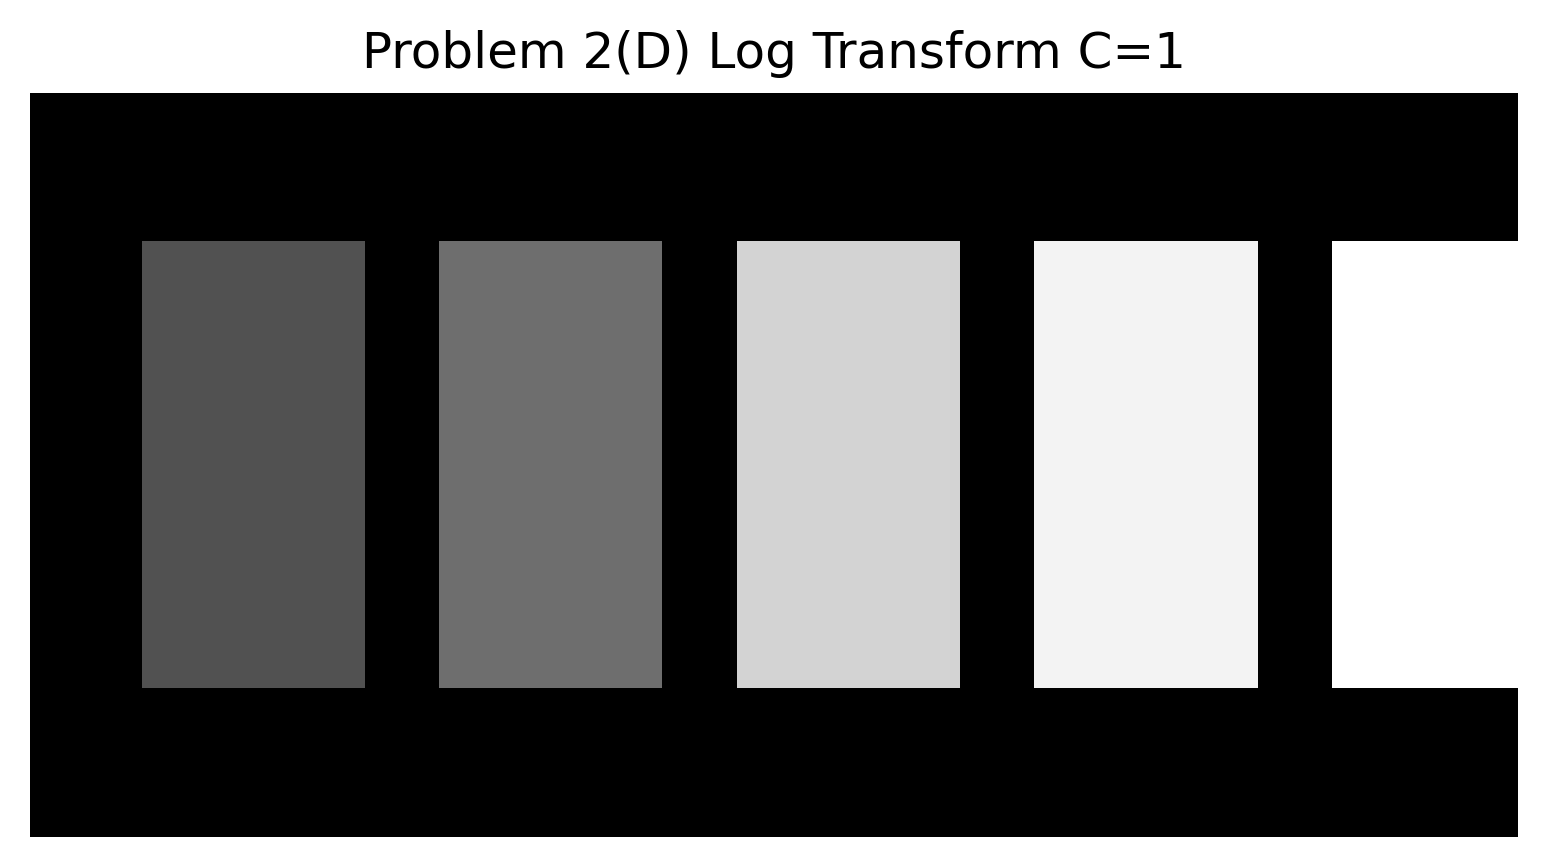
\includegraphics[width=0.49\textwidth]{plots/P2D_log_C_1.png}\hfill
			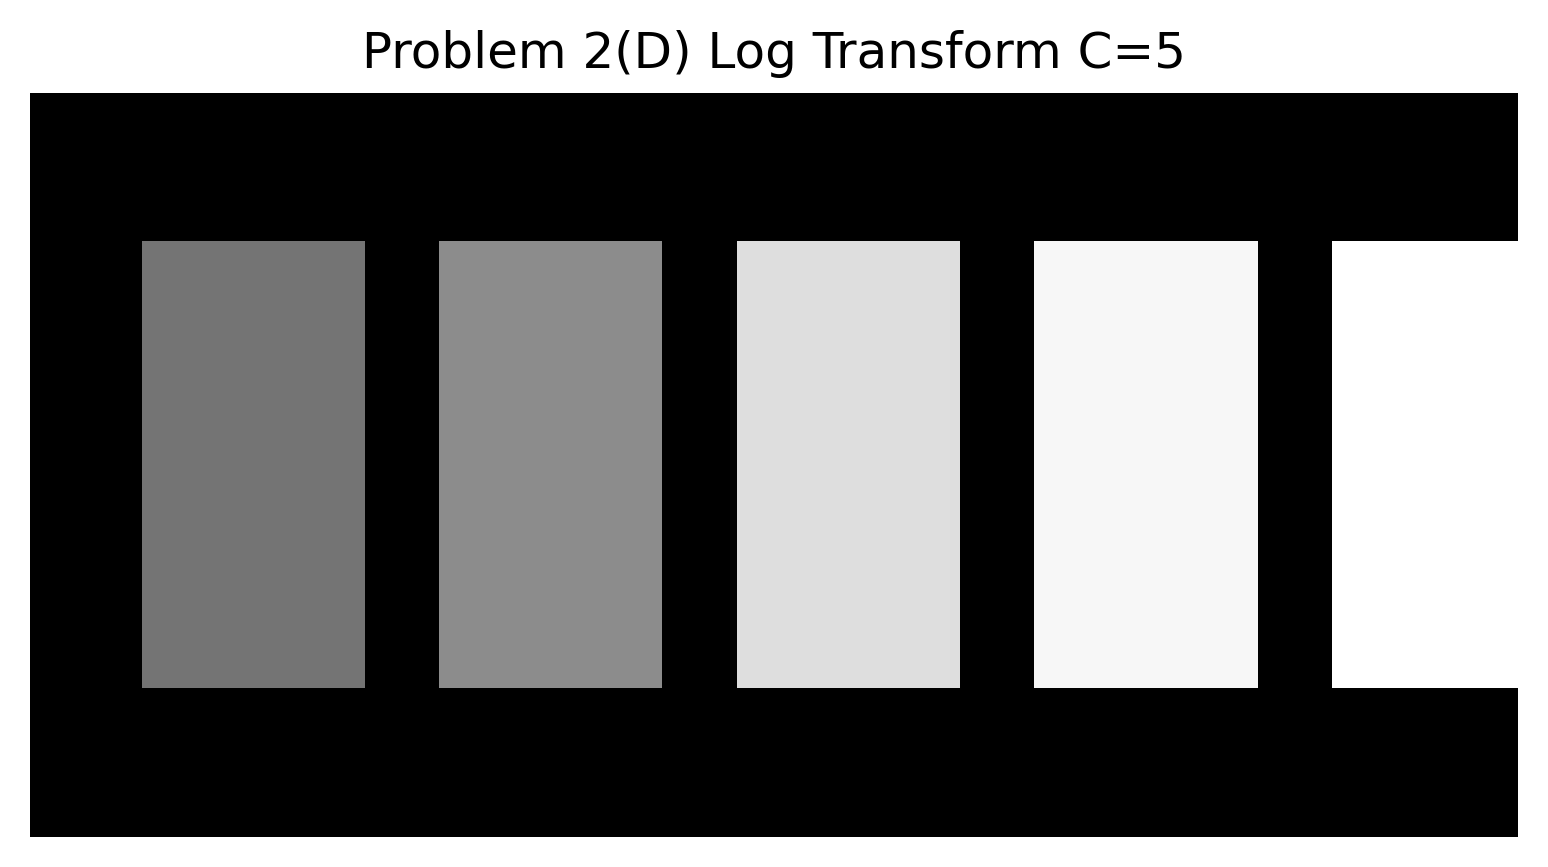
\includegraphics[width=0.49\textwidth]{plots/P2D_log_C_5.png}
			\caption{Problem 2(D): Log transform results for $C=1$ (left) and $C=5$ (right).}
		\end{figure}
		
		\begin{figure}[H]
			\centering
			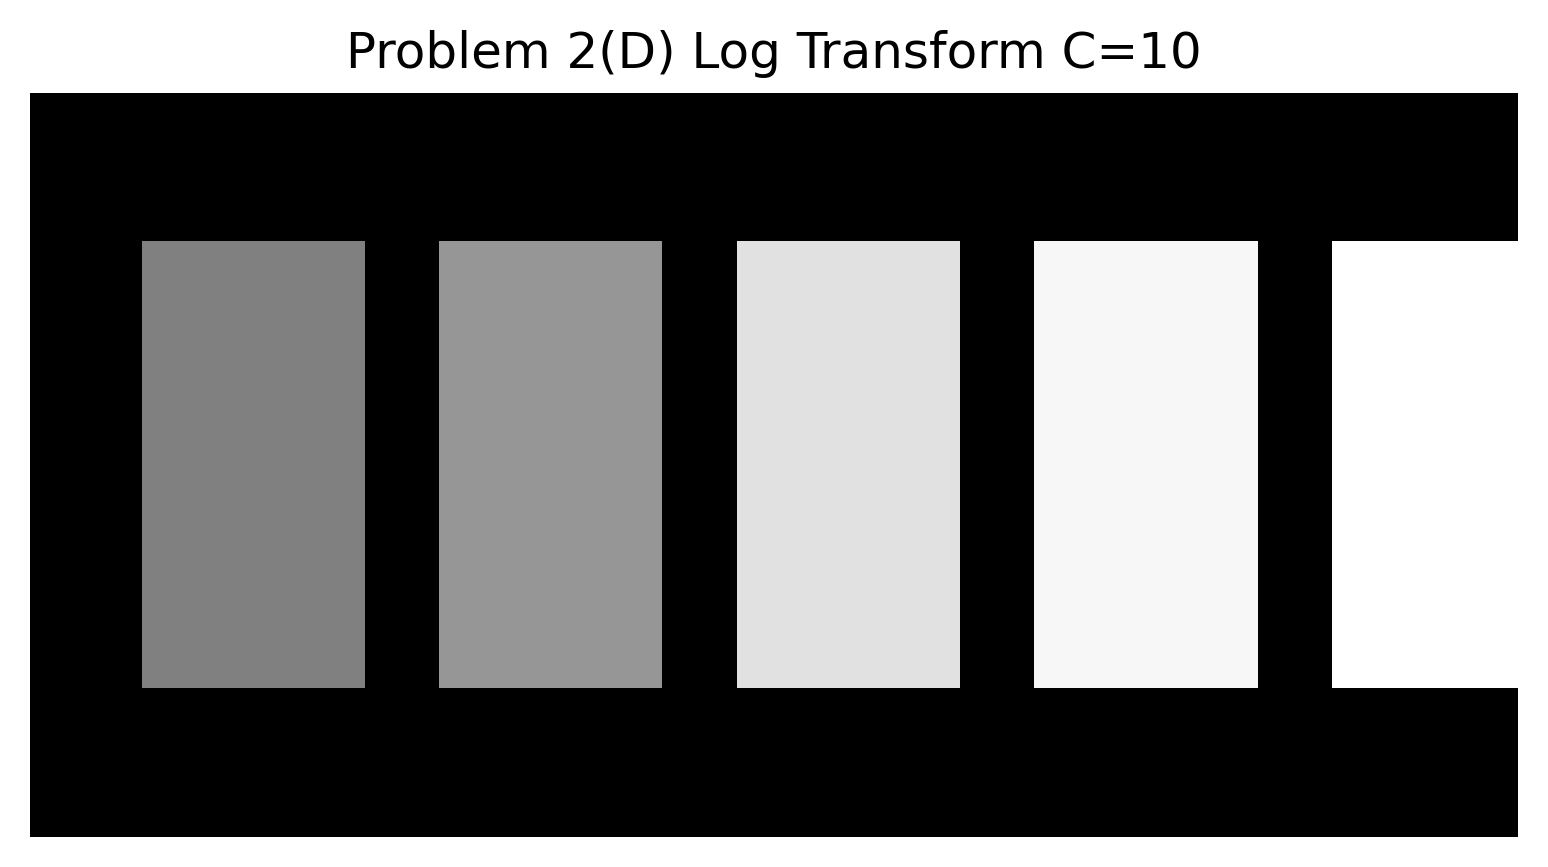
\includegraphics[width=0.49\textwidth]{plots/P2D_log_C_10.png}\hfill
			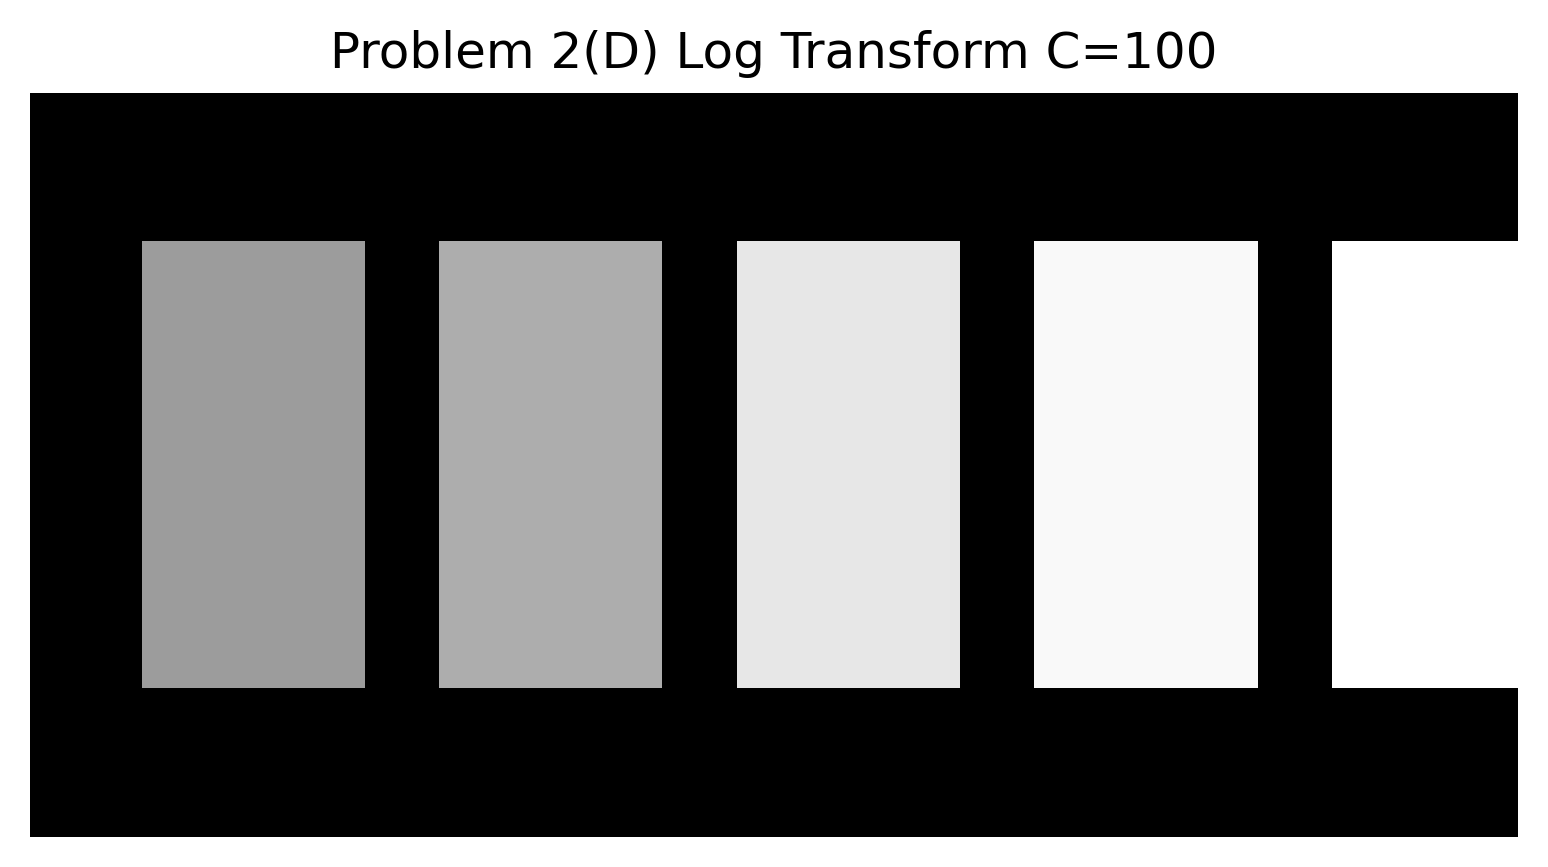
\includegraphics[width=0.49\textwidth]{plots/P2D_log_C_100.png}
			\caption{Problem 2(D): Log transform results for $C=10$ (left) and $C=100$ (right).}
		\end{figure}
		
		\textbf{Discussion:}
		Applying $\log(1 + C\cdot I)$ expands low intensities and compresses high intensities. As $C$ increases, the dark patches (5 and 10) become noticeably brighter relative to the background, improving their visibility. At the same time, the brightest patches (200 and 250) become more similar in brightness because the log function compresses large values, reducing their separation. For larger $C$ (e.g., 10 and 100), the overall appearance changes less dramatically because the transform becomes strongly compressive for the entire intensity range.
		
		\vspace{1em}
		
		% ===================== E =====================
		\item \textbf{Side-by-side comparisons and visibility table ($C=1,5,10,100$)}
		
		\begin{figure}[H]
			\centering
			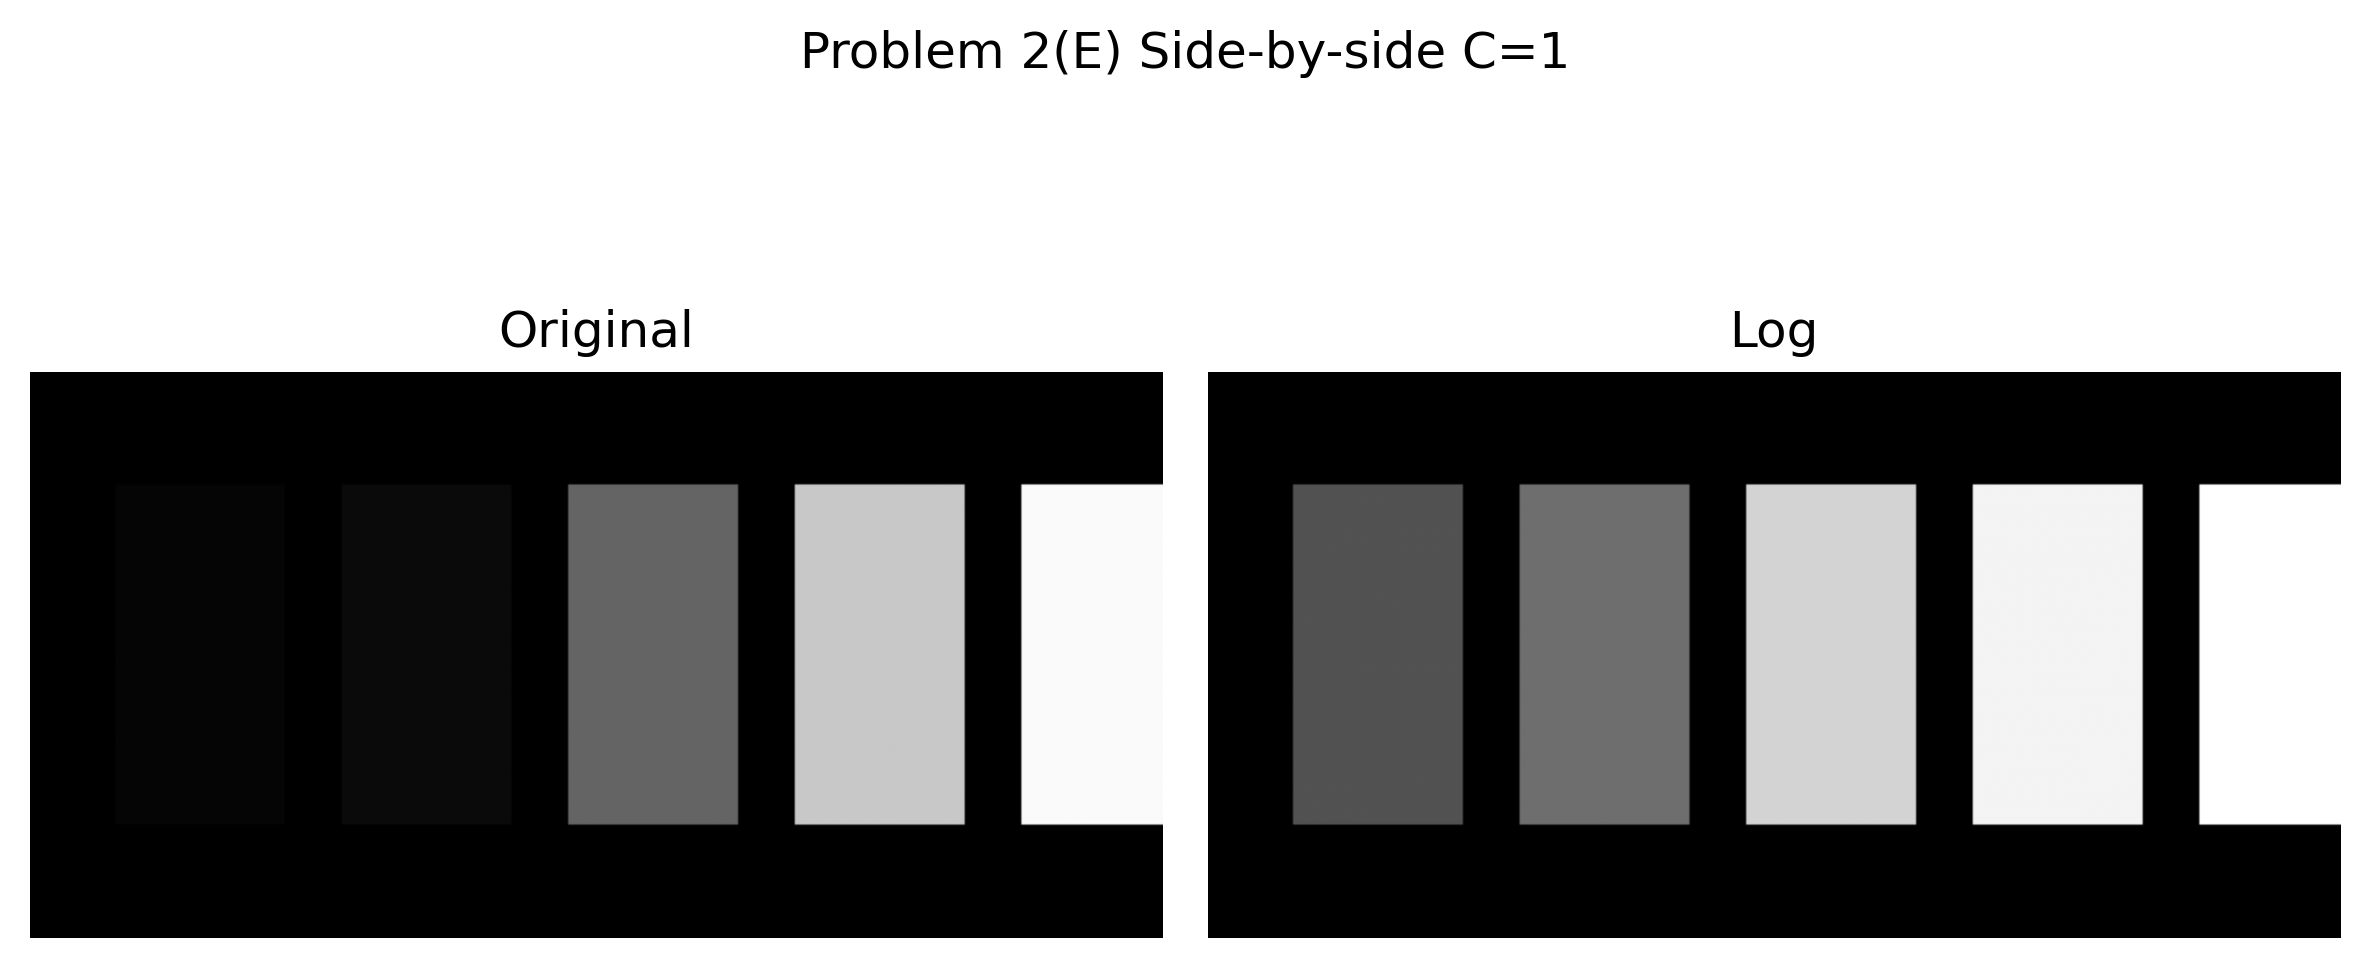
\includegraphics[width=0.95\textwidth]{plots/P2E_side_by_side_C_1.png}
			\caption{Problem 2(E): Side-by-side comparison for $C=1$ (Original vs Log).}
		\end{figure}
		
		\begin{figure}[H]
			\centering
			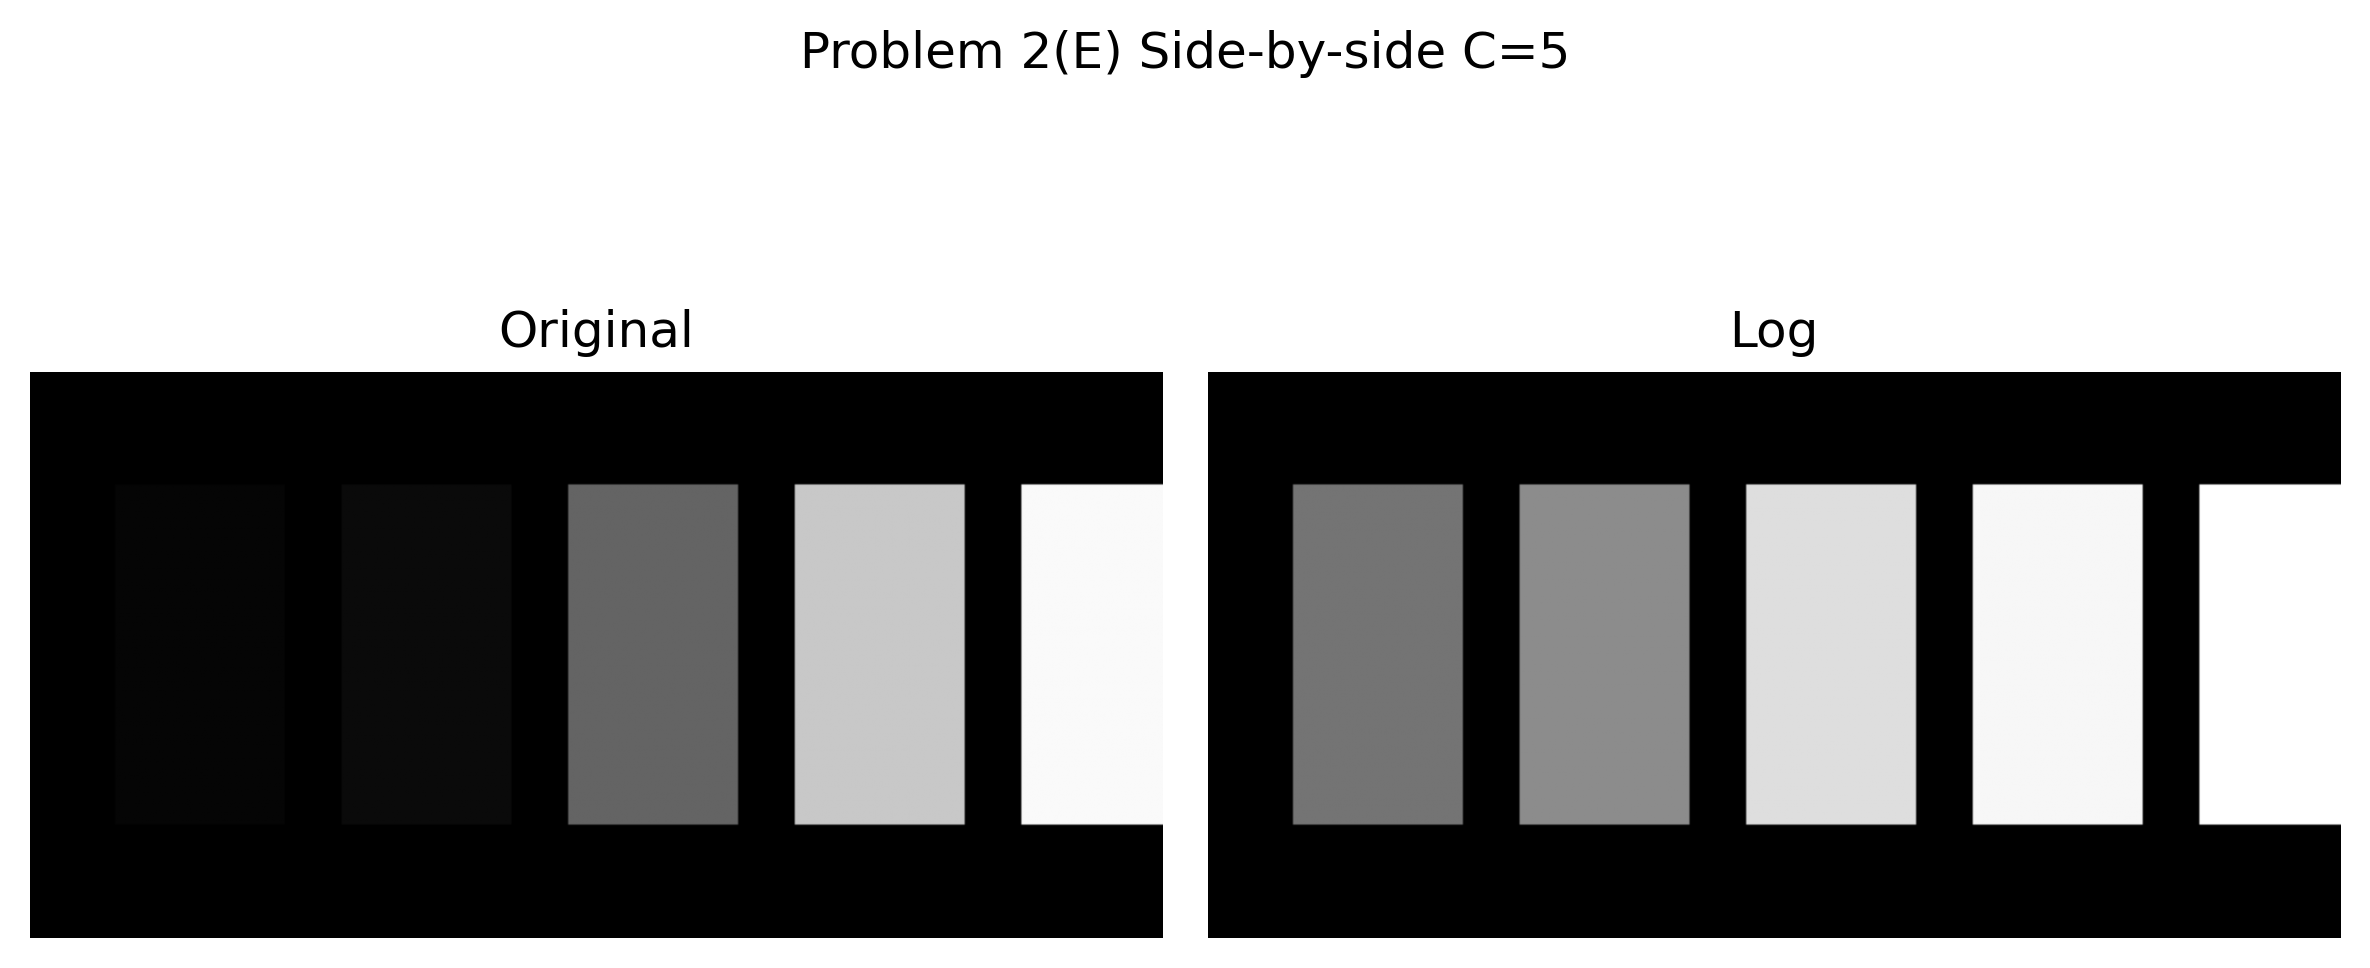
\includegraphics[width=0.95\textwidth]{plots/P2E_side_by_side_C_5.png}
			\caption{Problem 2(E): Side-by-side comparison for $C=5$ (Original vs Log).}
		\end{figure}
		
		\begin{figure}[H]
			\centering
			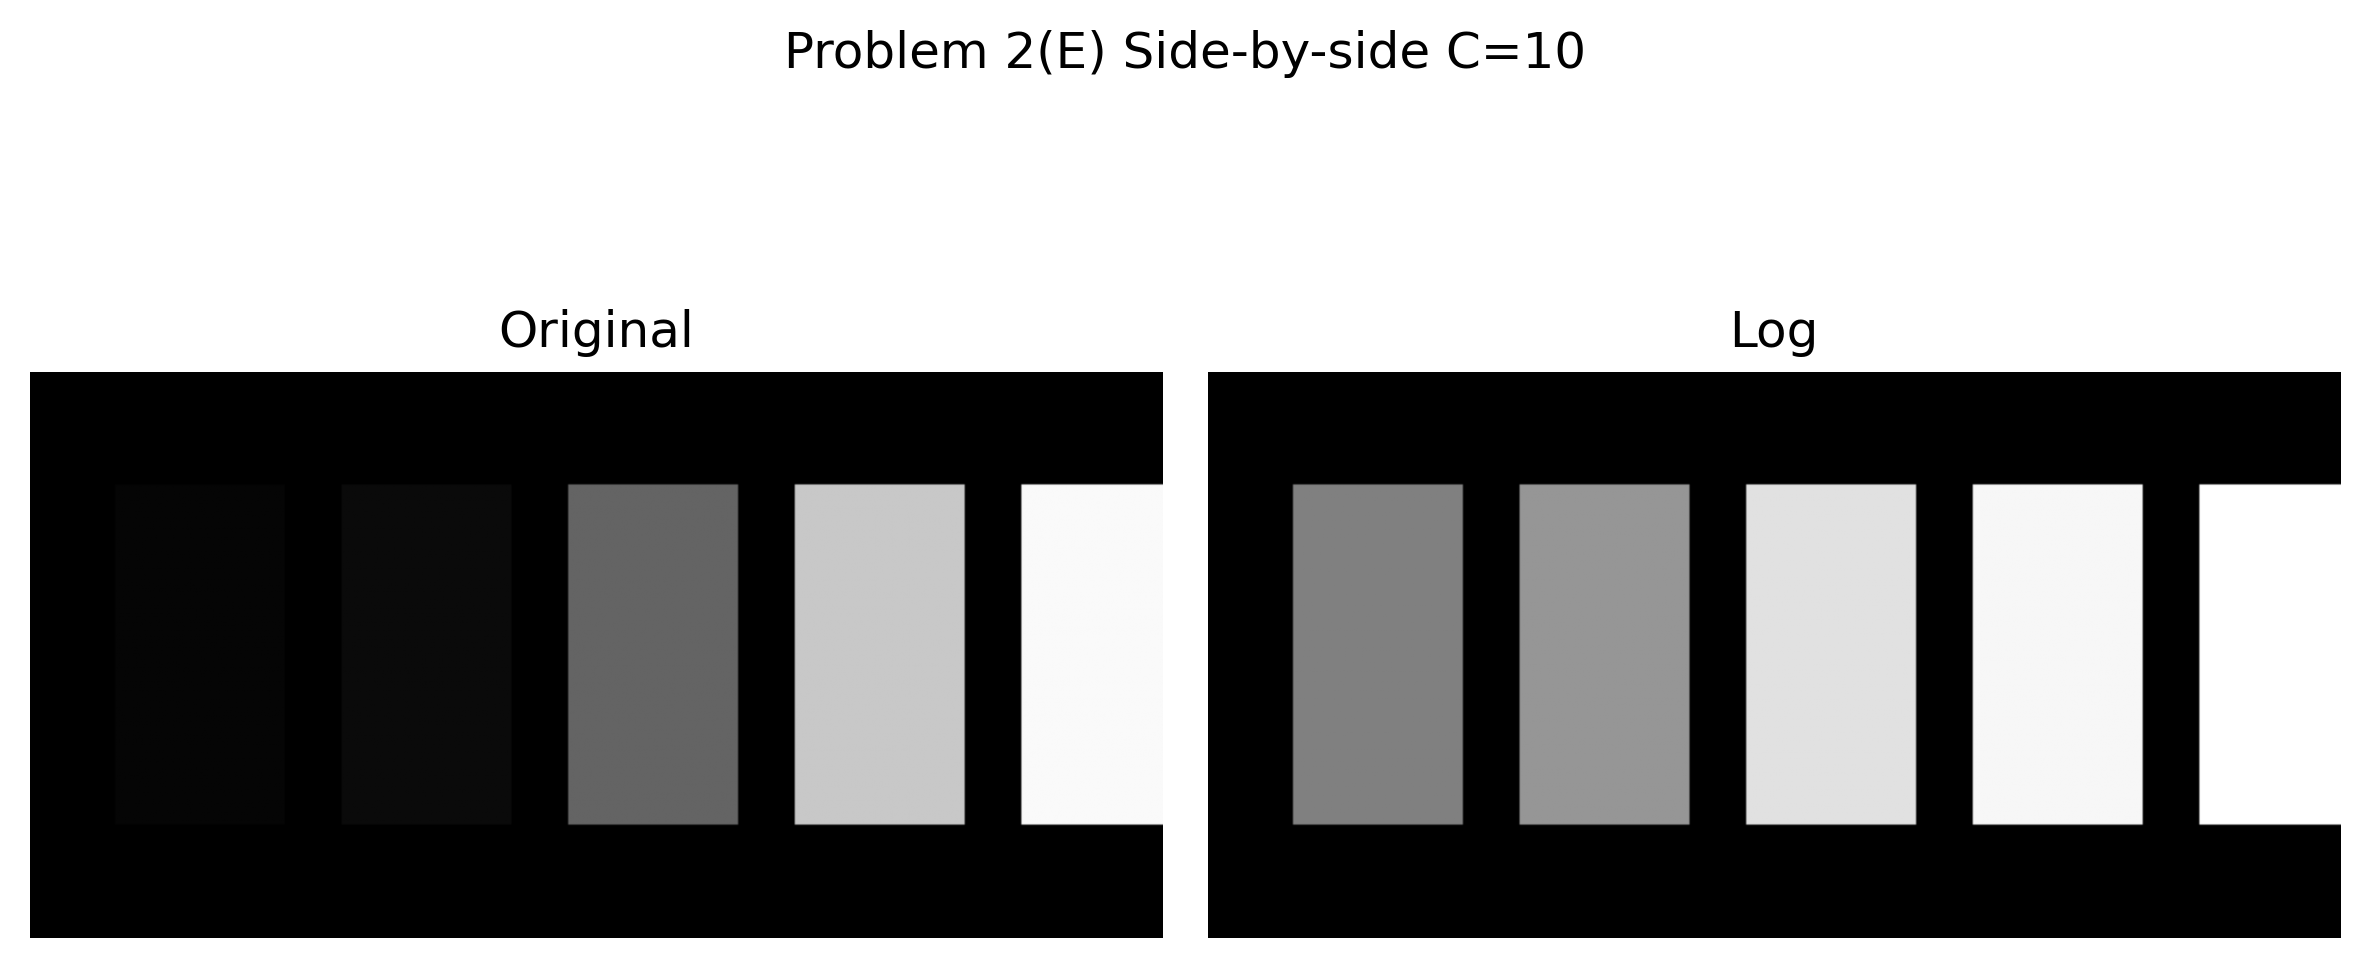
\includegraphics[width=0.95\textwidth]{plots/P2E_side_by_side_C_10.png}
			\caption{Problem 2(E): Side-by-side comparison for $C=10$ (Original vs Log).}
		\end{figure}
		
		\begin{figure}[H]
			\centering
			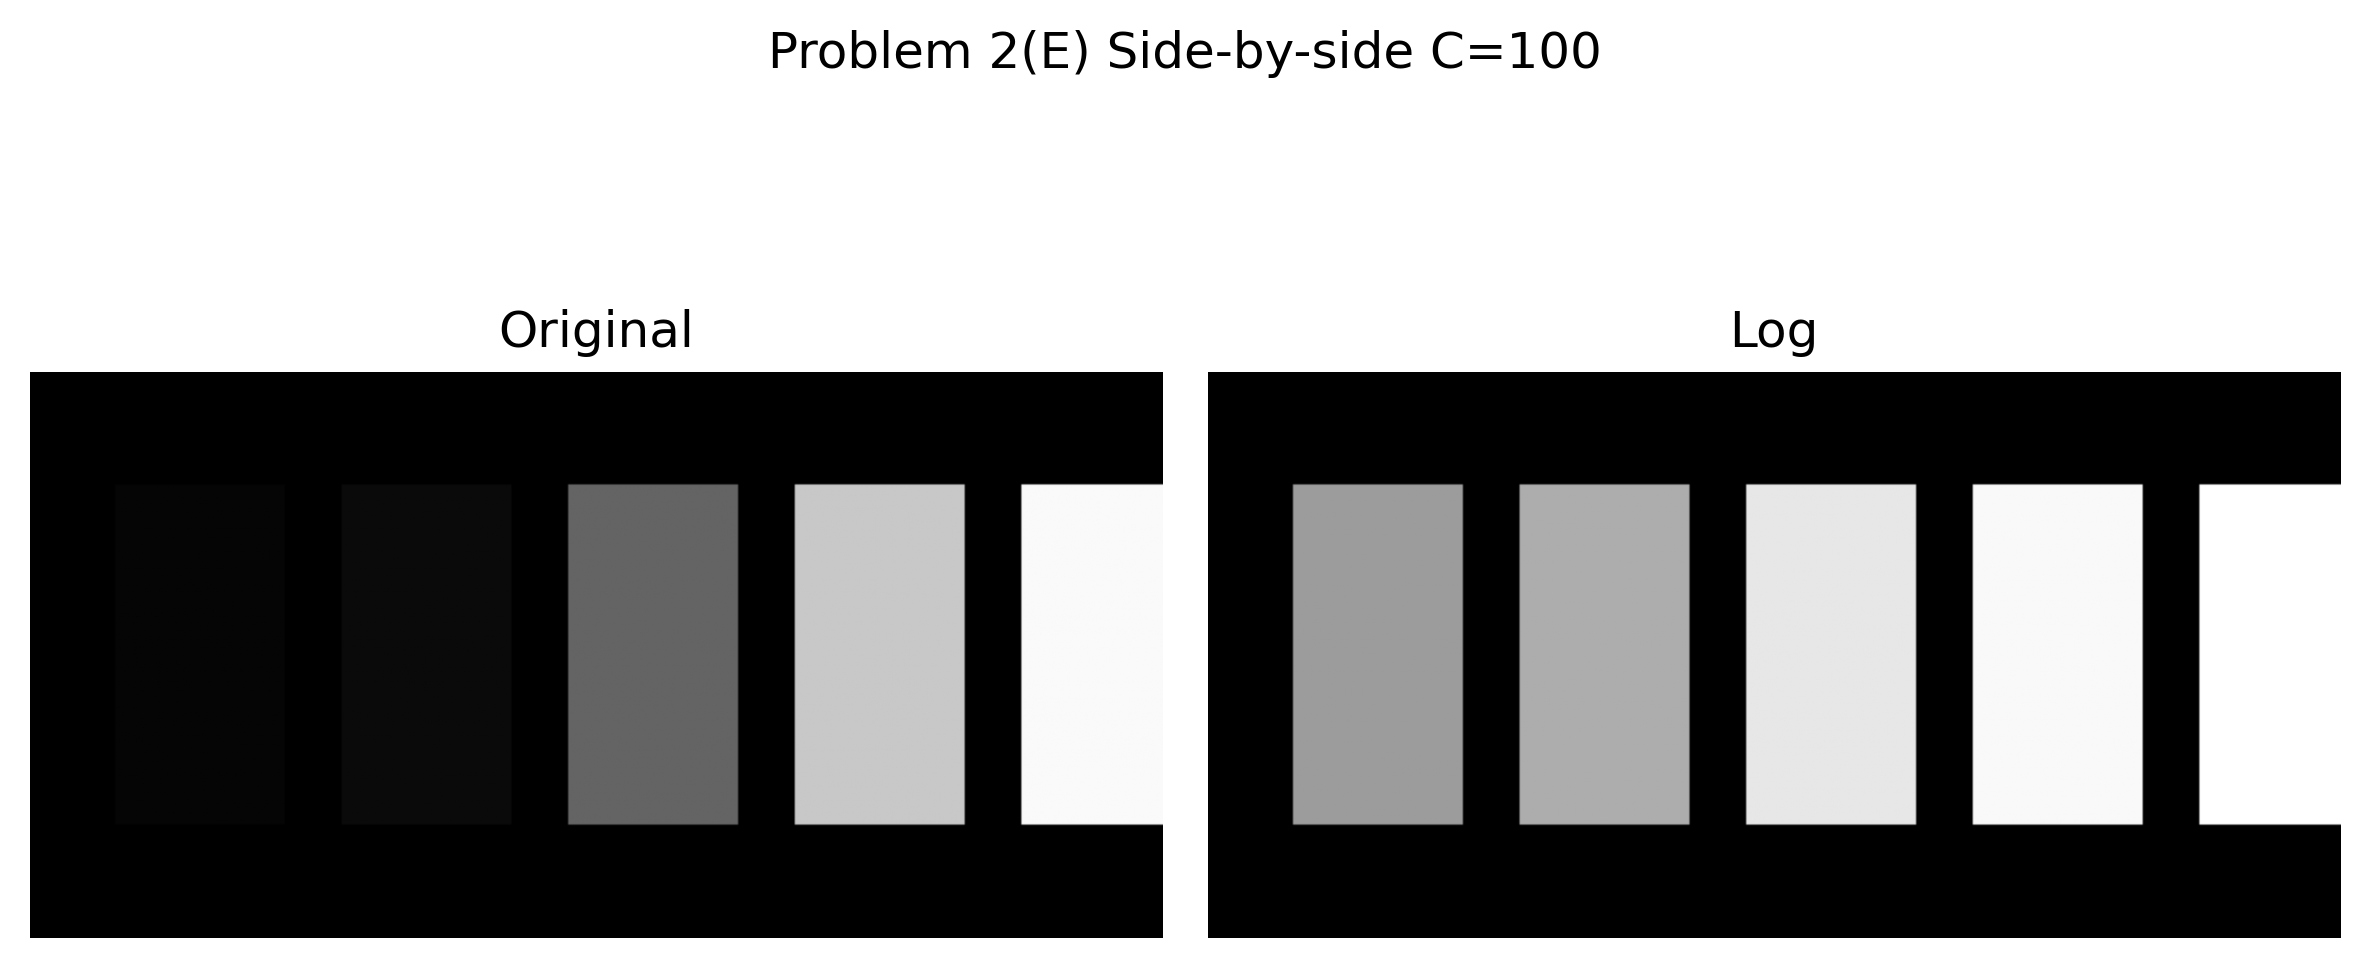
\includegraphics[width=0.95\textwidth]{plots/P2E_side_by_side_C_100.png}
			\caption{Problem 2(E): Side-by-side comparison for $C=100$ (Original vs Log).}
		\end{figure}
		
		\textbf{Discussion:}
		The side-by-side figures show that the log transform makes low-intensity patches easier to see (especially 5 and 10) as $C$ increases, because the transform expands small intensity differences. However, high-intensity patches (200 and 250) become less distinguishable from each other under larger $C$ due to compression at the bright end. The visibility scores in the table are based on perceived separability of each patch from the background and from nearby patches; different viewers may score slightly differently depending on patch size, spacing, and visual perception.
		
	\end{enumerate}
	
	\newpage
	
	% ---------------- Problem 3 ----------------
	\noindent\textbf{Problem 3. Images through activation functions (20 points)}
	
	Refer to the
	\href{https://colab.research.google.com/github/pattichis/AIML/blob/main/Session_8_Create_videos.ipynb#scrollTo=vhSh4F_an5j4}{image patches example}
	and
	\href{https://github.com/pattichis/AIML/blob/main/Session_14_Activation_Functions.ipynb}{activation functions tutorial}.
	
	\begin{enumerate}[label=\textbf{(\alph*)}, leftmargin=1.2cm]
		\item Create an image with zero background and constant patches of 5 and 100.
		\item Show how a ReLU with proper bias eliminates the lower-brightness patch.
		\item Show how a Sigmoid with proper bias reduces the lower-brightness patch.
	\end{enumerate}
	
	\vspace{1em}
	\noindent\textbf{Solution.}
	
	\begin{enumerate}[label=\textbf{(\alph*)}, leftmargin=1.2cm]
		
		% ===================== (a) =====================
		\item \textbf{Image with zero background and constant patches}
		
		\begin{figure}[H]
			\centering
			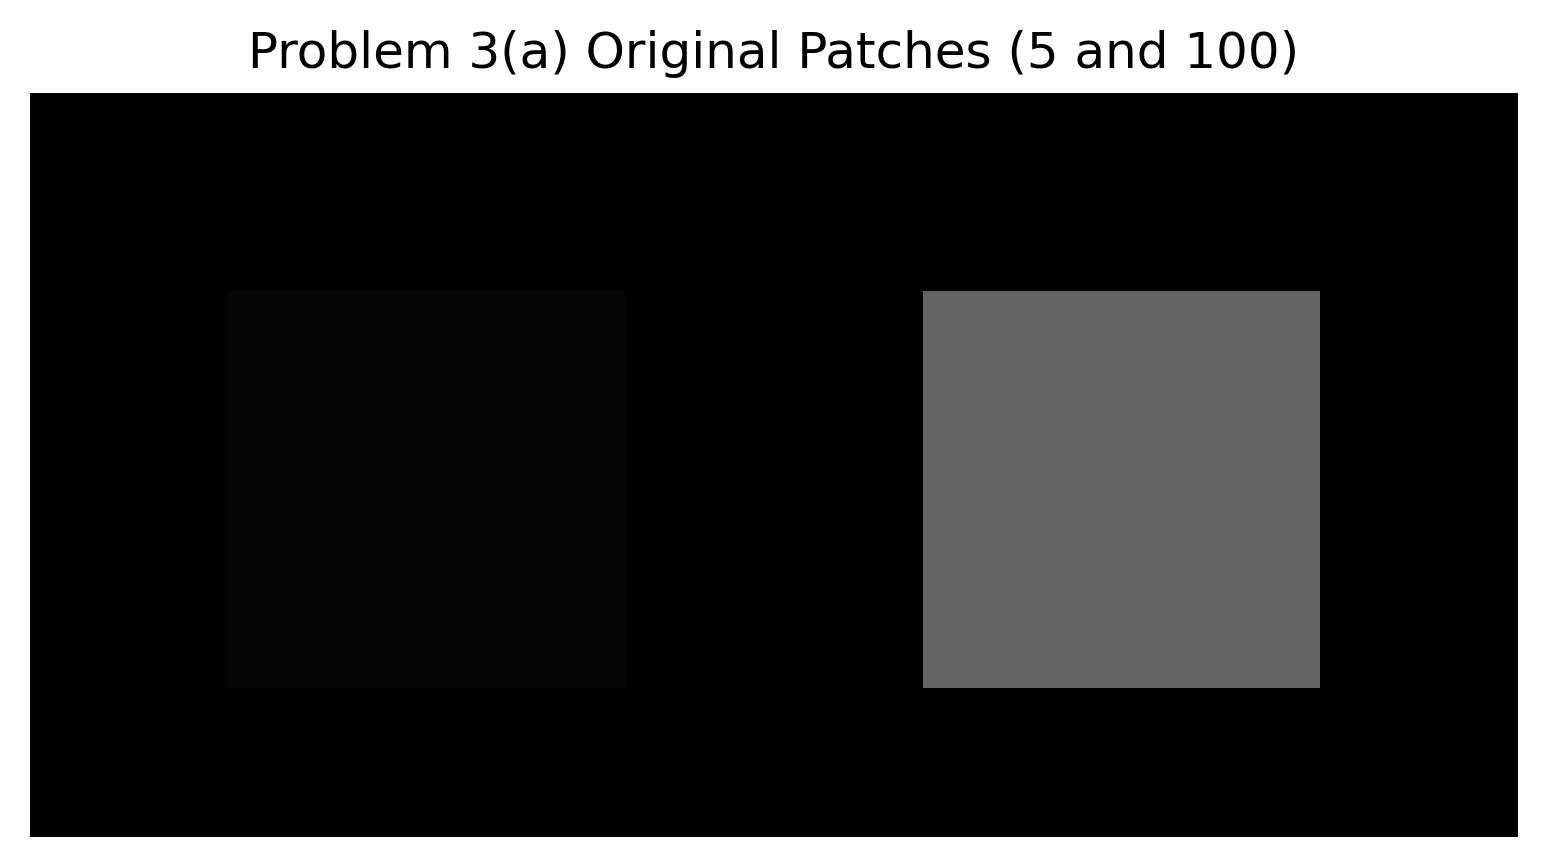
\includegraphics[width=0.75\textwidth]{plots/P3A_original.png}
			\caption{Problem 3(a): Original image with patches of intensity 5 and 100 on a zero background.}
		\end{figure}
		
		\textbf{Discussion:}
		The image contains two constant-intensity patches placed on a black background. The left patch has intensity 5 and appears very dark, while the right patch has intensity 100 and is clearly brighter. This serves as the baseline image to observe how different activation functions modify pixel intensities.
		
		
		\vspace{1em}
		
		% ===================== (b) =====================
		\item \textbf{ReLU with proper bias}
		
		\begin{figure}[H]
			\centering
			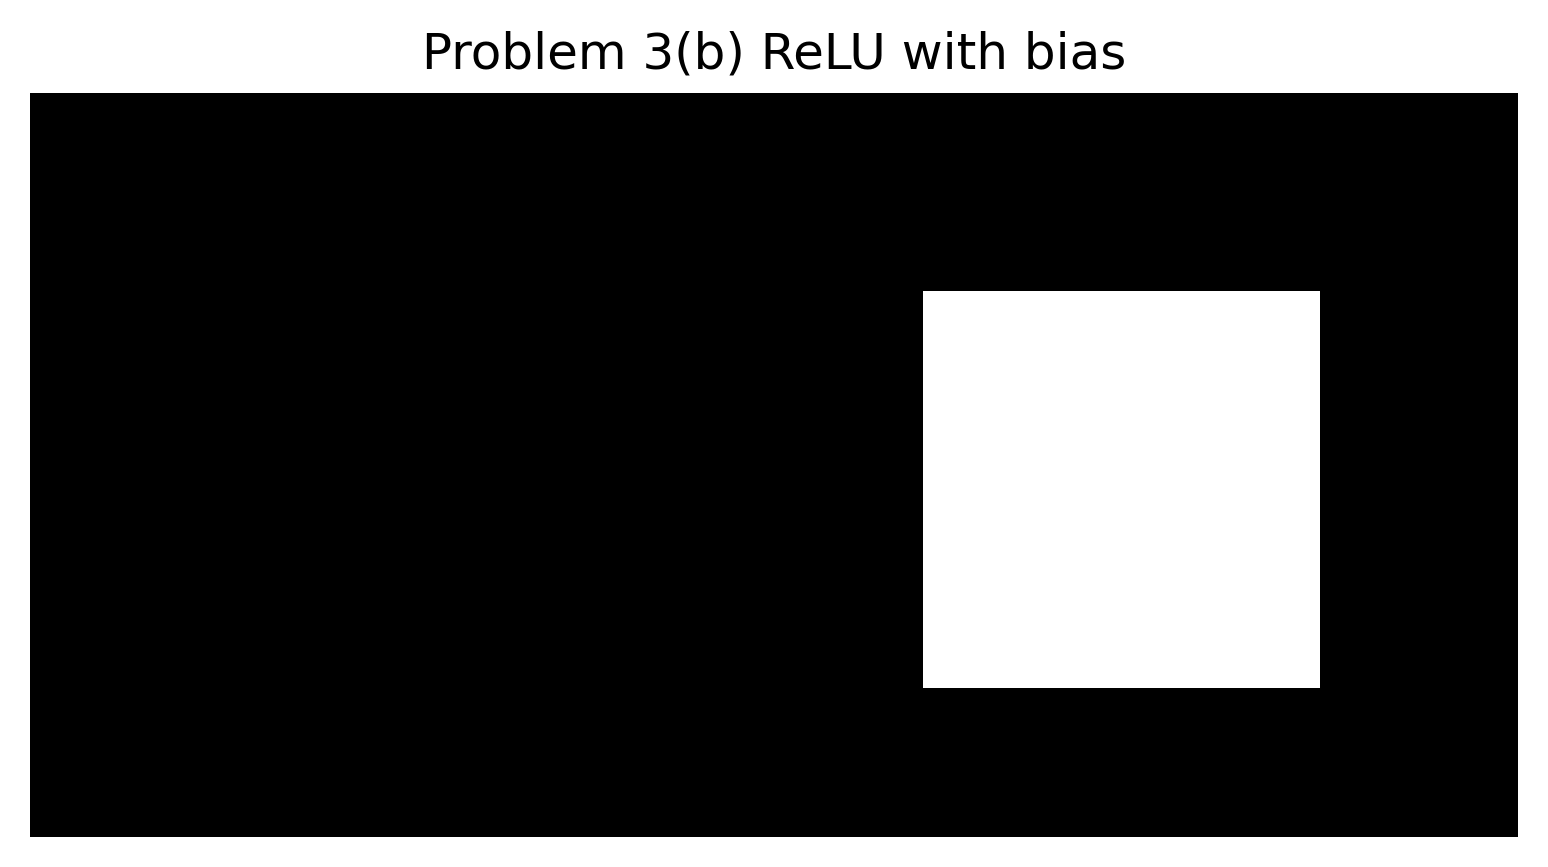
\includegraphics[width=0.75\textwidth]{plots/P3B_relu.png}
			\caption{Problem 3(b): ReLU activation with bias applied.}
		\end{figure}
		
		\textbf{Discussion:}
		A ReLU activation was applied after subtracting a positive bias from the image intensities. The low-intensity patch (value 5) becomes negative after the bias shift and is clipped to zero by the ReLU, effectively eliminating it. The higher-intensity patch (value 100) remains positive and is preserved. Thus, ReLU acts like a hard threshold that completely removes low-brightness regions while keeping stronger signals.
		
		
		\vspace{1em}
		
		% ===================== (c) =====================
		\item \textbf{Sigmoid with proper bias}
		
		\begin{figure}[H]
			\centering
			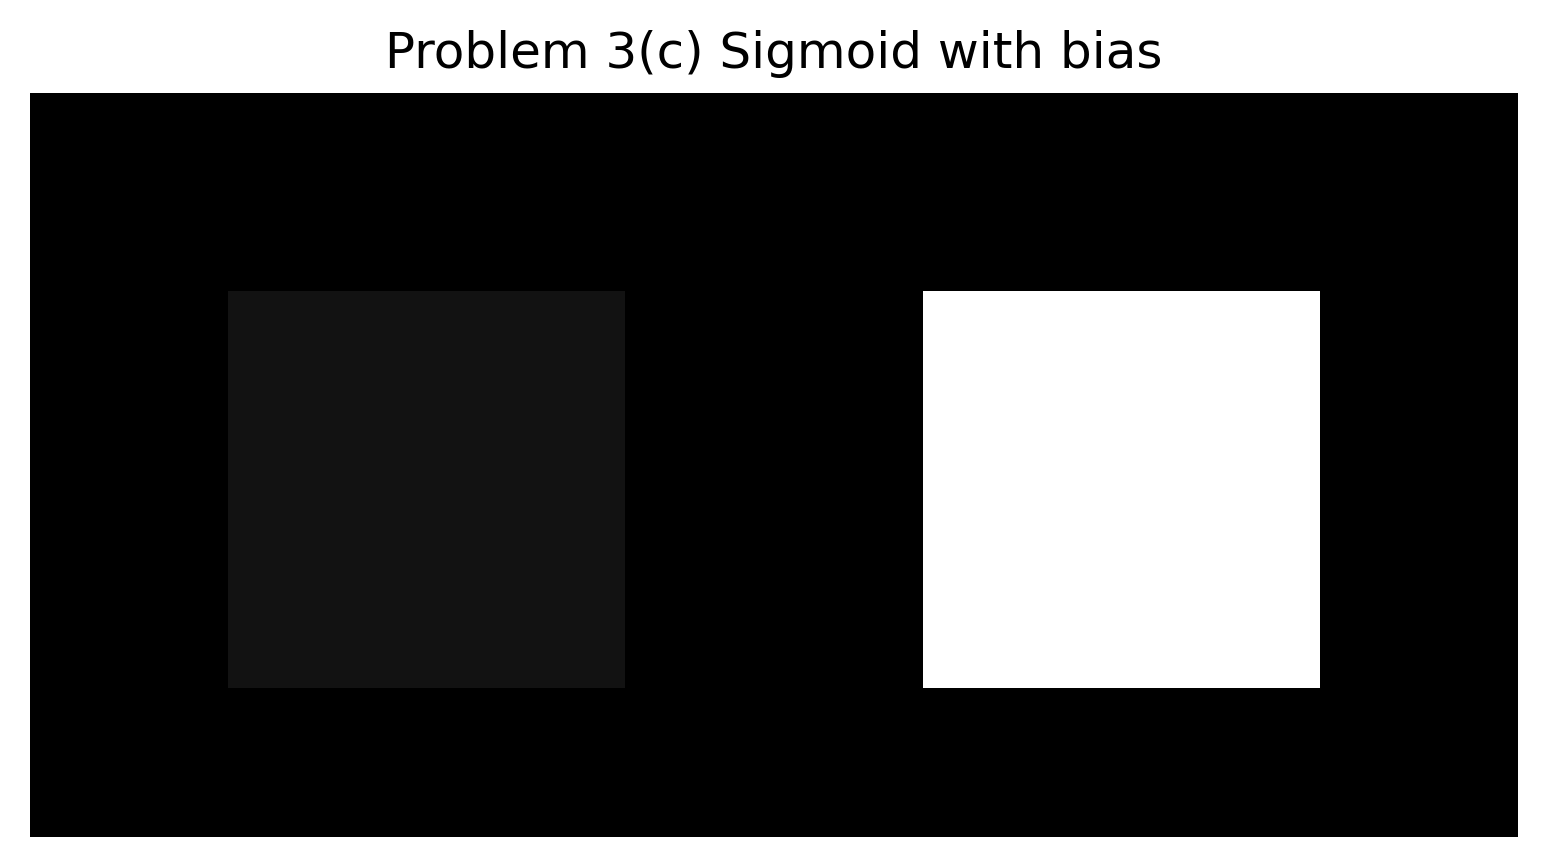
\includegraphics[width=0.75\textwidth]{plots/P3C_sigmoid.png}
			\caption{Problem 3(c): Sigmoid activation with bias applied.}
		\end{figure}
		
		\textbf{Discussion:}
		The sigmoid activation produces a smooth, nonlinear compression rather than a hard cutoff. After applying a bias, the lower-intensity patch is mapped close to zero but not completely removed, so it appears faint instead of disappearing. The higher-intensity patch maps near one and remains bright. Compared to ReLU, the sigmoid reduces low intensities gradually instead of eliminating them, resulting in softer contrast transitions.
		
	\end{enumerate}
	
	\newpage
	
	% ---------------- Problem 4 ----------------
	\noindent\textbf{Problem 4. Max Pooling and downsampling (40 points)}
	
	For this problem, refer to the 
	\href{https://github.com/pattichis/AIML/blob/main/Session_13_Max_Pooling.ipynb}{max pooling example}.\\
	
	Here, we want to use the greyscale definitions of dilation and erosion:
	
	\[
	\begin{aligned}
		& O[i, j] = \text{Dilation}(I, S)[i, j] = \max_{(i', j') \in S+(i, j)} I[i', j']\\
		& O[i, j] = \text{Erosion}(I, S)[i, j]  = \min_{(i', j') \in S+(i, j)} I[i', j']\\
		\text{where:} & \\
		& (i', j') \in S+(i, j) = \left\{(i', j') \mid (i', j') = (i, j) + (d_1, d_2), \ (d_1, d_2) \in S \right\}
	\end{aligned}
	\]
	
	Also, note that for grayscale morphology, dilation is equivalent to max pooling without downsampling.\\
	
	\begin{enumerate}[label=\textbf{\Alph*.}, leftmargin=1.2cm]
		
		\item Show that max pooling by an $N \times N$ window, stride $N$, followed by $N \times N$ downsampling preserves the maximum value in the original window.
		
		\item Create an image with zero background, a rectangular patch with a value of 100 with a smaller rectangular hole with value $=0$.
		
		\item Use the rolling-ball analogy from dilation to estimate the output from dilating with a $2 \times 2$. Show your work using pencil and paper.
		
		\item Verify your example using max pooling in Python.
		
		\item Demonstrate how you can increase the size of the max pooling to eliminate the smaller rectangular hole. What is the minimum square size of your kernel? Derive a mathematical expression.
		
		\item Suppose that the hole still appears after the max pooling operation. Sketch a diagram to show how it can disappear during the downsampling process.
		
		\item Suppose that the input image is multiplied by $-1$. Then apply the max pooling operation without downsampling. What is the relationship of the output image to applying an erosion to the input image?
		
		\item How can you implement erosion using max pooling and multiplication by a constant?
		
	\end{enumerate}
	
	\vspace{1em}
	\noindent\textbf{Solution.}
	
	\begin{enumerate}[label=\textbf{\Alph*.}, leftmargin=1.2cm]
		
		\item \textbf{Max pooling + downsampling preserves the maximum.}\\
		Let $I$ be an image and consider any non-overlapping $N\times N$ block $B$ of pixels. Max pooling with kernel $N\times N$ and stride $N$ outputs one value per block:
		\[
		P[u,v] \;=\; \max_{(i,j)\in B_{u,v}} I[i,j].
		\]
		Since stride $N$ creates one pooled value per block, the pooled output already \emph{is} the maximum of each original $N\times N$ block. If we then perform $N\times N$ downsampling (i.e., keep exactly one representative per $N\times N$ region), we are still keeping that block-maximum value. Therefore, the maximum value in each original $N\times N$ window is preserved.
		
		\item \textbf{Image with patch=100 and hole=0.}\\
		Construct an image with background $0$, a rectangular region set to $100$, and a smaller rectangular sub-region (hole) set back to $0$ inside the $100$ patch. This creates a bright object with a dark hole.
		
		\item \textbf{Rolling-ball analogy (estimate dilation with $2\times 2$).}\\
		Dilation with a $2\times 2$ structuring element replaces each output pixel with the maximum over its local $2\times 2$ neighborhood. Intuitively, a “rolling ball” (max operator) passes over the image: wherever the $2\times 2$ window touches the bright $100$ patch, the output becomes $100$. Thus, the bright region expands by about one pixel (depending on anchor convention) and the hole shrinks because many $2\times 2$ windows overlapping the hole still include surrounding $100$ pixels.
		
		\item \textbf{Verify dilation using max pooling in Python.}\\
		Grayscale dilation (with a square structuring element) is equivalent to max pooling with \emph{stride $1$} (no downsampling). So, using \texttt{torch.nn.functional.max\_pool2d} with \texttt{kernel\_size=2} and \texttt{stride=1} reproduces the dilation result.
		
		\item \textbf{Increase kernel size to eliminate the hole; minimum kernel and formula.}\\
		A sufficient condition to completely fill a rectangular hole of height $h$ and width $w$ (inside a constant-bright region) is that the max window is large enough so that every window whose center lies in the hole still overlaps at least one $100$ pixel outside the hole. A common rule-of-thumb for a square kernel is
		\[
		k_{\min} \approx 2\left\lceil\frac{\max(h,w)}{2}\right\rceil + 1
		\]
		(using odd $k$ for a symmetric “radius” interpretation).\\
		In our measured example, the hole was $16\times 20$ and this rule gives $k_{\min}=21$, while brute force (stride=1, no padding) found the smallest kernel that fills the hole was $k=17$ :contentReference[oaicite:0]{index=0}. The difference comes from implementation details (anchor/placement, boundary handling, and the fact that “must overlap outside” can be satisfied with a smaller kernel depending on how the window is positioned relative to the hole).
		
		\item \textbf{How downsampling can remove a remaining hole (sketch idea).}\\
		Even if a tiny hole remains after dilation/max pooling (stride=1), downsampling with stride $N$ can “miss” that hole if the sampling grid does not land on it. For example, if the remaining hole is only 1 pixel wide, a stride-2 sampling that keeps only every other pixel may select only surrounding $100$ pixels, making the hole disappear in the downsampled image.
		
		\item \textbf{Multiply by $-1$, apply max pooling, relate to erosion.}\\
		Erosion is the \emph{minimum} over a neighborhood:
		\[
		\text{Erosion}(I,S)[i,j] = \min_{(i',j')\in S+(i,j)} I[i',j'].
		\]
		But $\min$ can be written using $\max$ via negation:
		\[
		\min(\mathcal{N}) = -\max(-\mathcal{N}).
		\]
		So erosion can be computed as:
		\[
		\text{Erosion}(I,S) \;=\; -\,\text{Dilation}(-I,S),
		\]
		and since dilation $\equiv$ max pooling (stride=1), this becomes:
		\[
		\text{Erosion}(I,S) \;=\; -\,\text{MaxPool}(-I).
		\]
		
		\item \textbf{Implement erosion using max pooling and multiplication.}\\
		To erode an image $I$ with a $k\times k$ square structuring element:
		\[
		E = -\text{MaxPool2D}(-I;\; \text{kernel}=k,\; \text{stride}=1).
		\]
		That is: multiply the input by $-1$, apply max pooling with stride 1 (no downsampling), then multiply by $-1$ again.
		
	\end{enumerate}
	
	\newpage
	
	% ---------------- Problem 5 ----------------
	\noindent\textbf{Problem 5. Image segmentation using histograms (40 points)}
	
	For this problem, use 
	\href{https://github.com/pattichis/AIML/blob/main/Session_7_2_image_analysis_with_color.ipynb}{image analysis session}.\\
	
	Adjust the thresholds to detect: \\
	\quad A. The bear \\
	\quad B. Skin color (yellow-like), and \\
	\quad C. Clothes for the minion. \\
	
	You will need to provide screenshots for each case that show the histograms, input image, binary mask, and output image.
	
	\vspace{1em}
	\noindent\textbf{Solution.}
	
	For this problem, I used RGB histograms and simple channel-wise thresholding (inequalities on the R, G, and B channels) to create a binary mask:
	\[
	\text{Mask}(i,j)=
	\begin{cases}
		1, & R_{\min}\le R(i,j)\le R_{\max}\ \wedge\ G_{\min}\le G(i,j)\le G_{\max}\ \wedge\ B_{\min}\le B(i,j)\le B_{\max}\\
		0, & \text{otherwise.}
	\end{cases}
	\]
	Then I produced the output image by keeping only pixels where the mask is 1 (and setting the rest to black). The thresholds were adjusted by inspecting the RGB histograms and selecting ranges that isolate the desired object color.
	
	\vspace{0.75em}
	\noindent\textbf{(a) Detect the bear.}
	The bear is brown, which corresponds to mid-range intensities with relatively higher red content compared to blue in many pixels. I tuned the thresholds so the binary mask highlights the bear region while suppressing the white background and most of the minion body. The resulting detected region area was \textbf{7750 pixels} (from the binary mask figure). The output image shows the bear (and some nearby brown-ish pixels) preserved while the background is removed.
	
	\begin{center}
		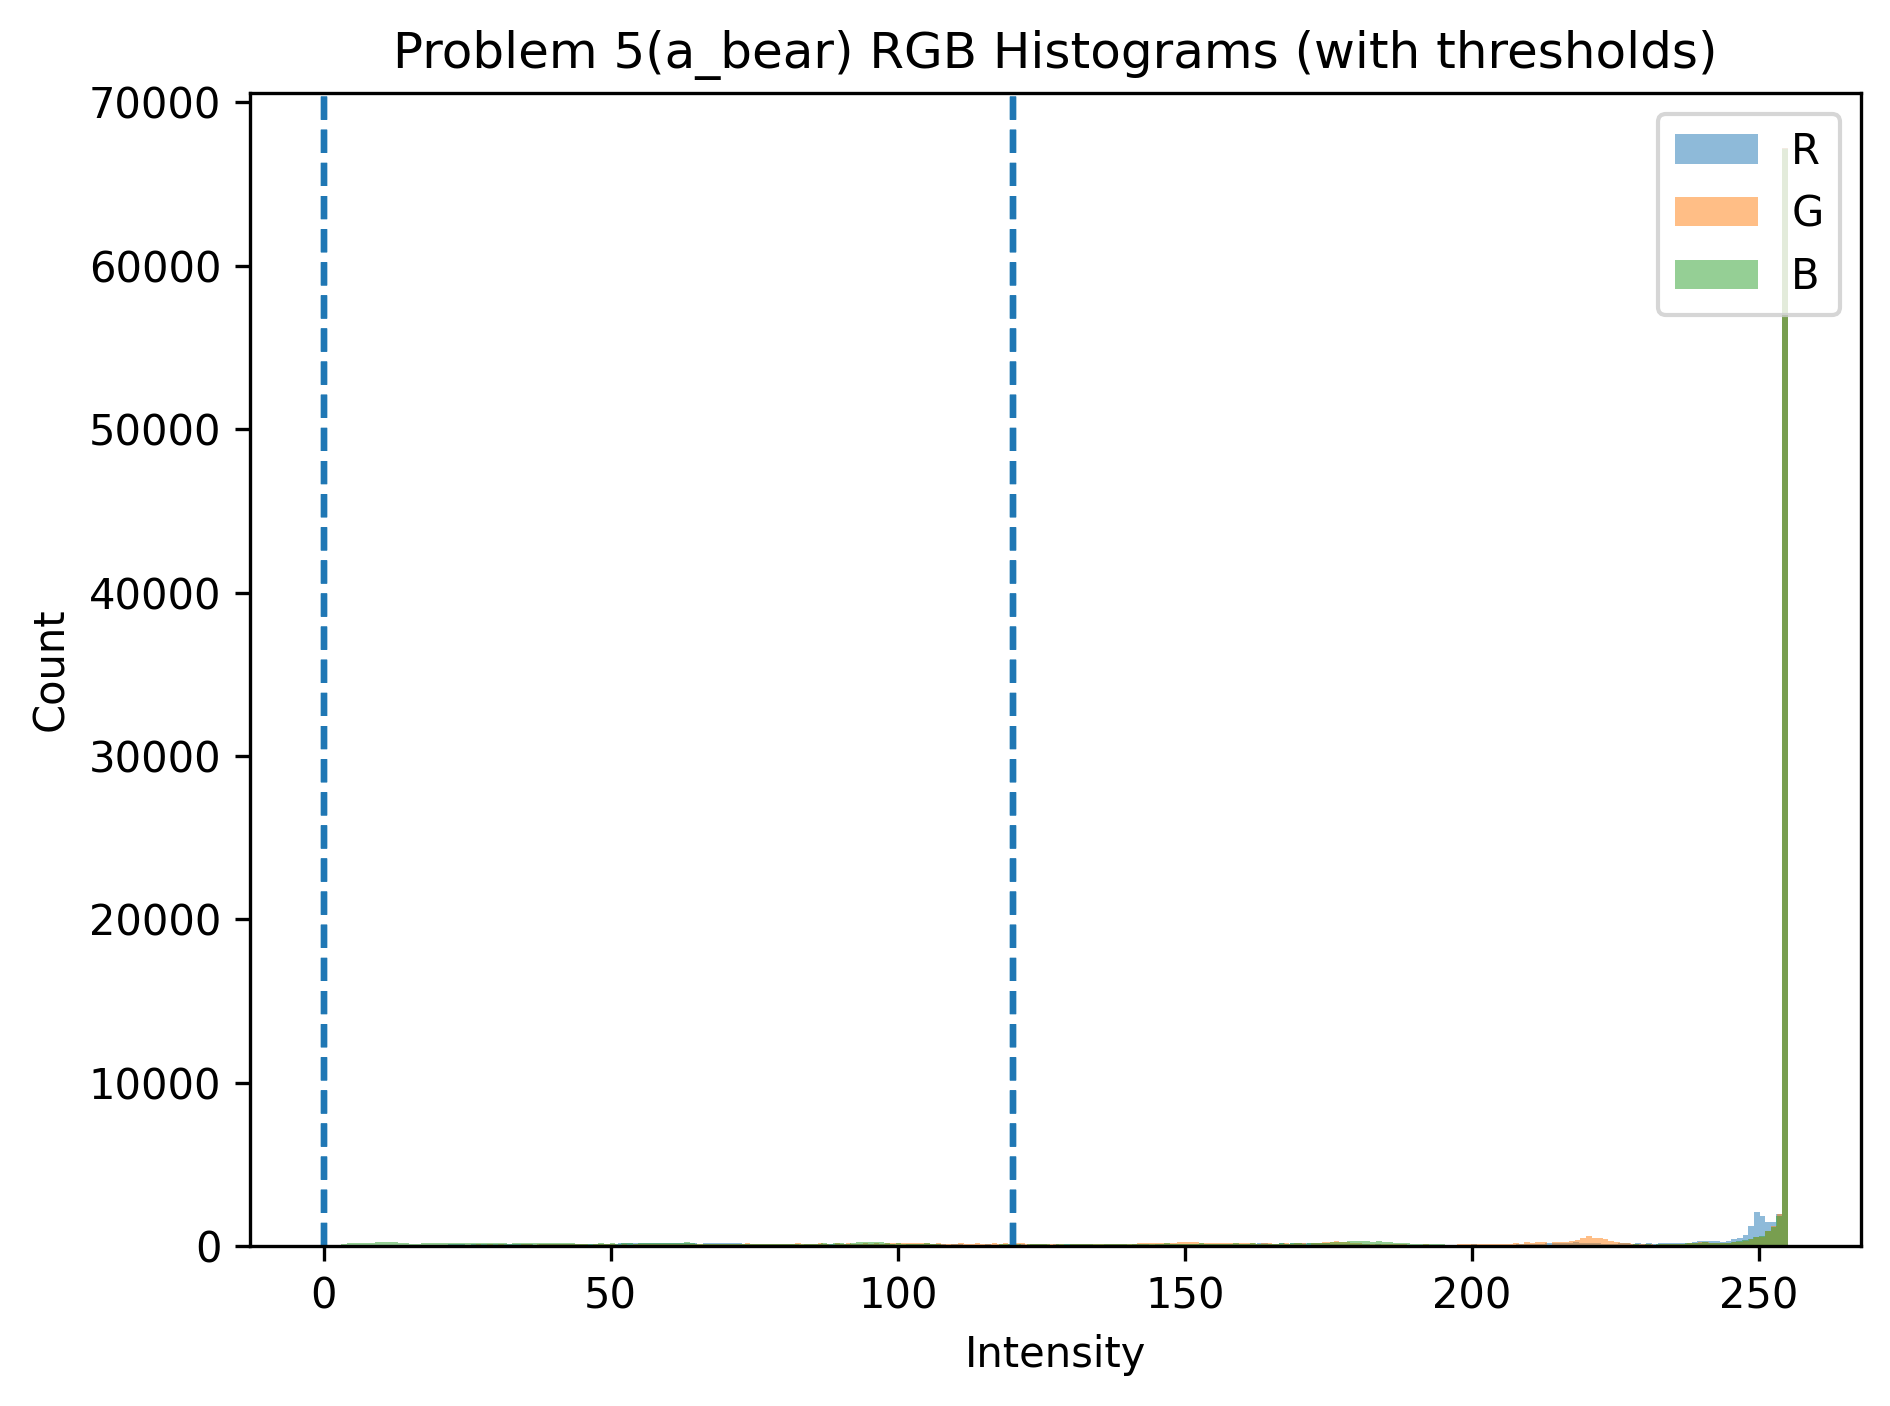
\includegraphics[width=0.45\textwidth]{plots/P5_a_bear_hist.png}\hfill
		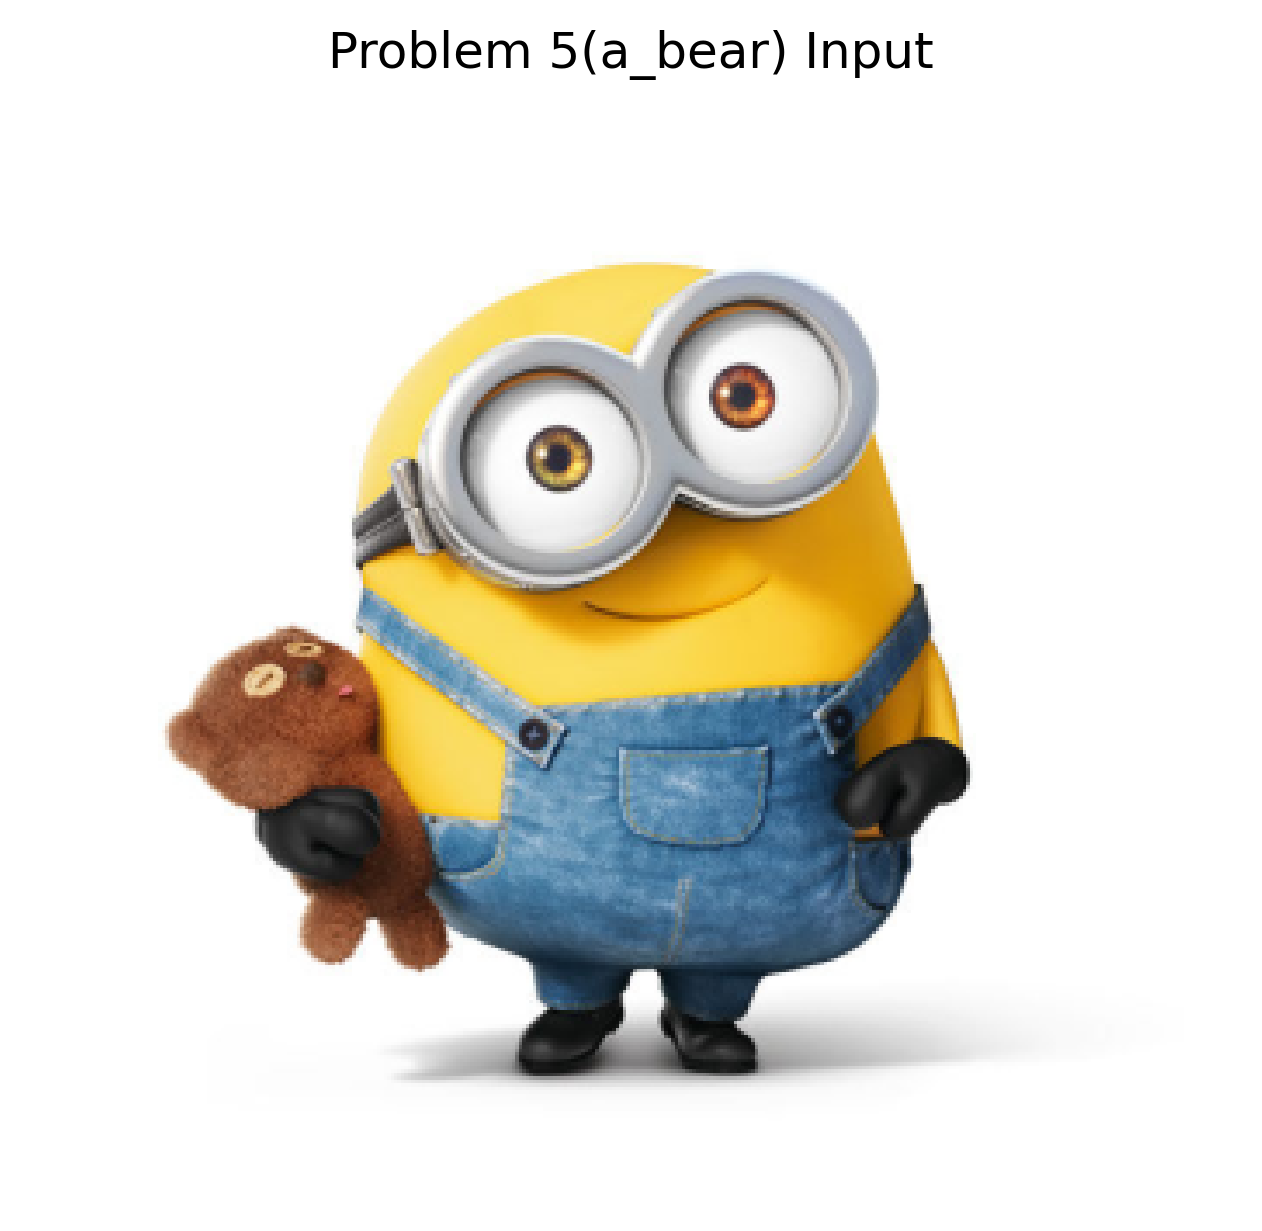
\includegraphics[width=0.45\textwidth]{plots/P5_a_bear_input.png}\\[0.5em]
		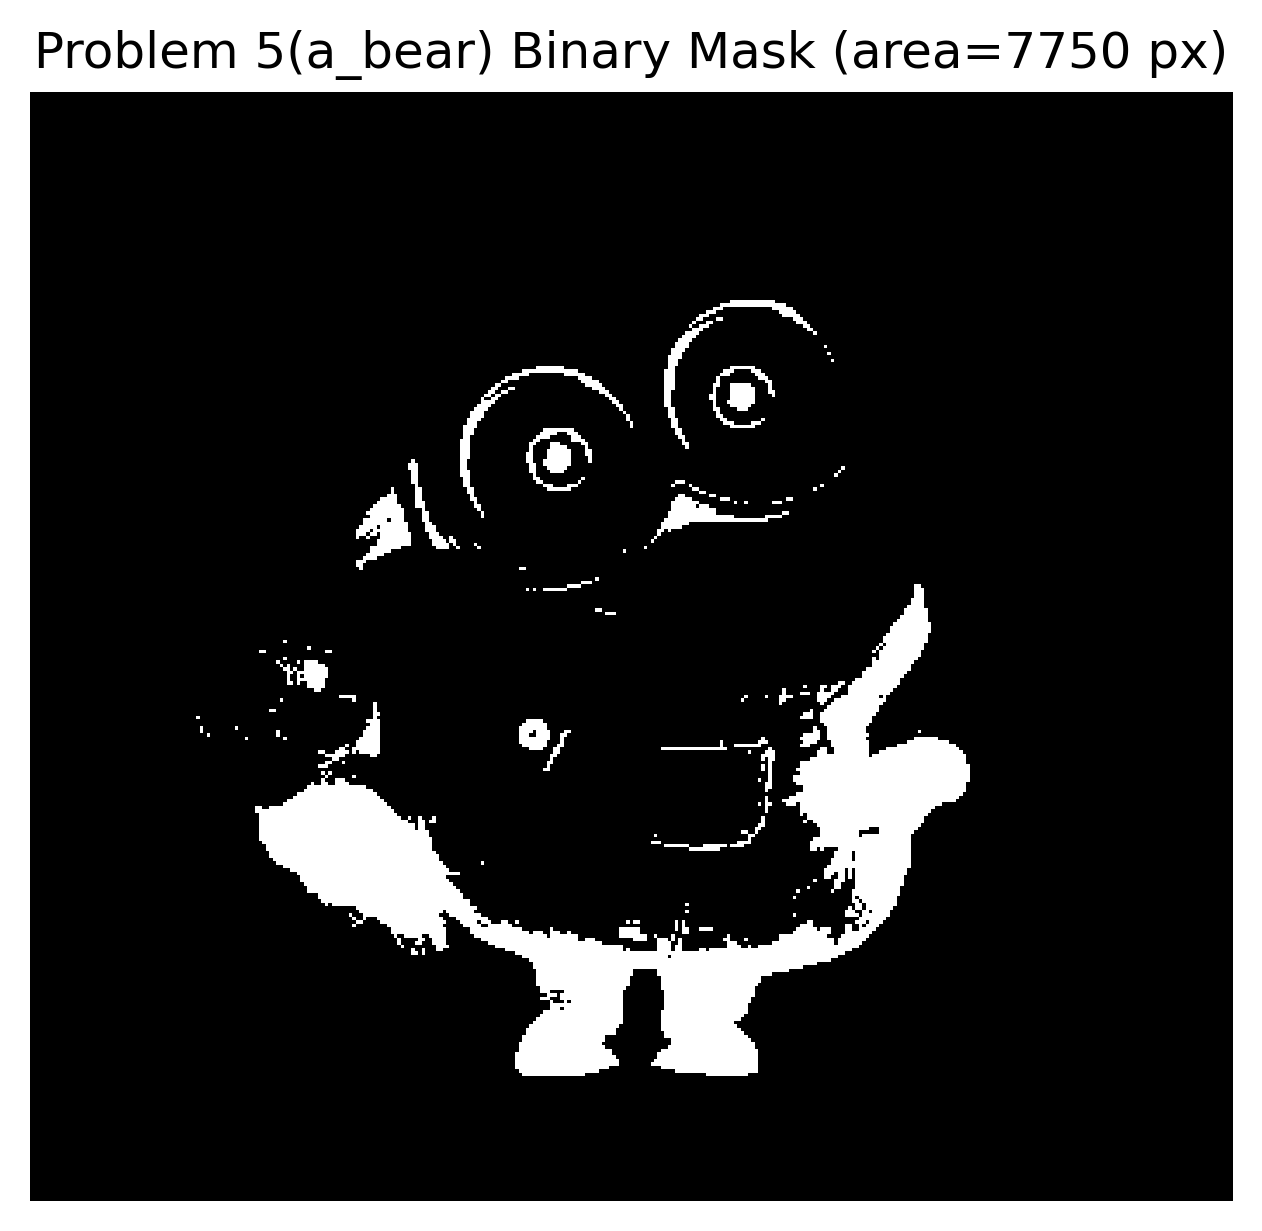
\includegraphics[width=0.45\textwidth]{plots/P5_a_bear_mask.png}\hfill
		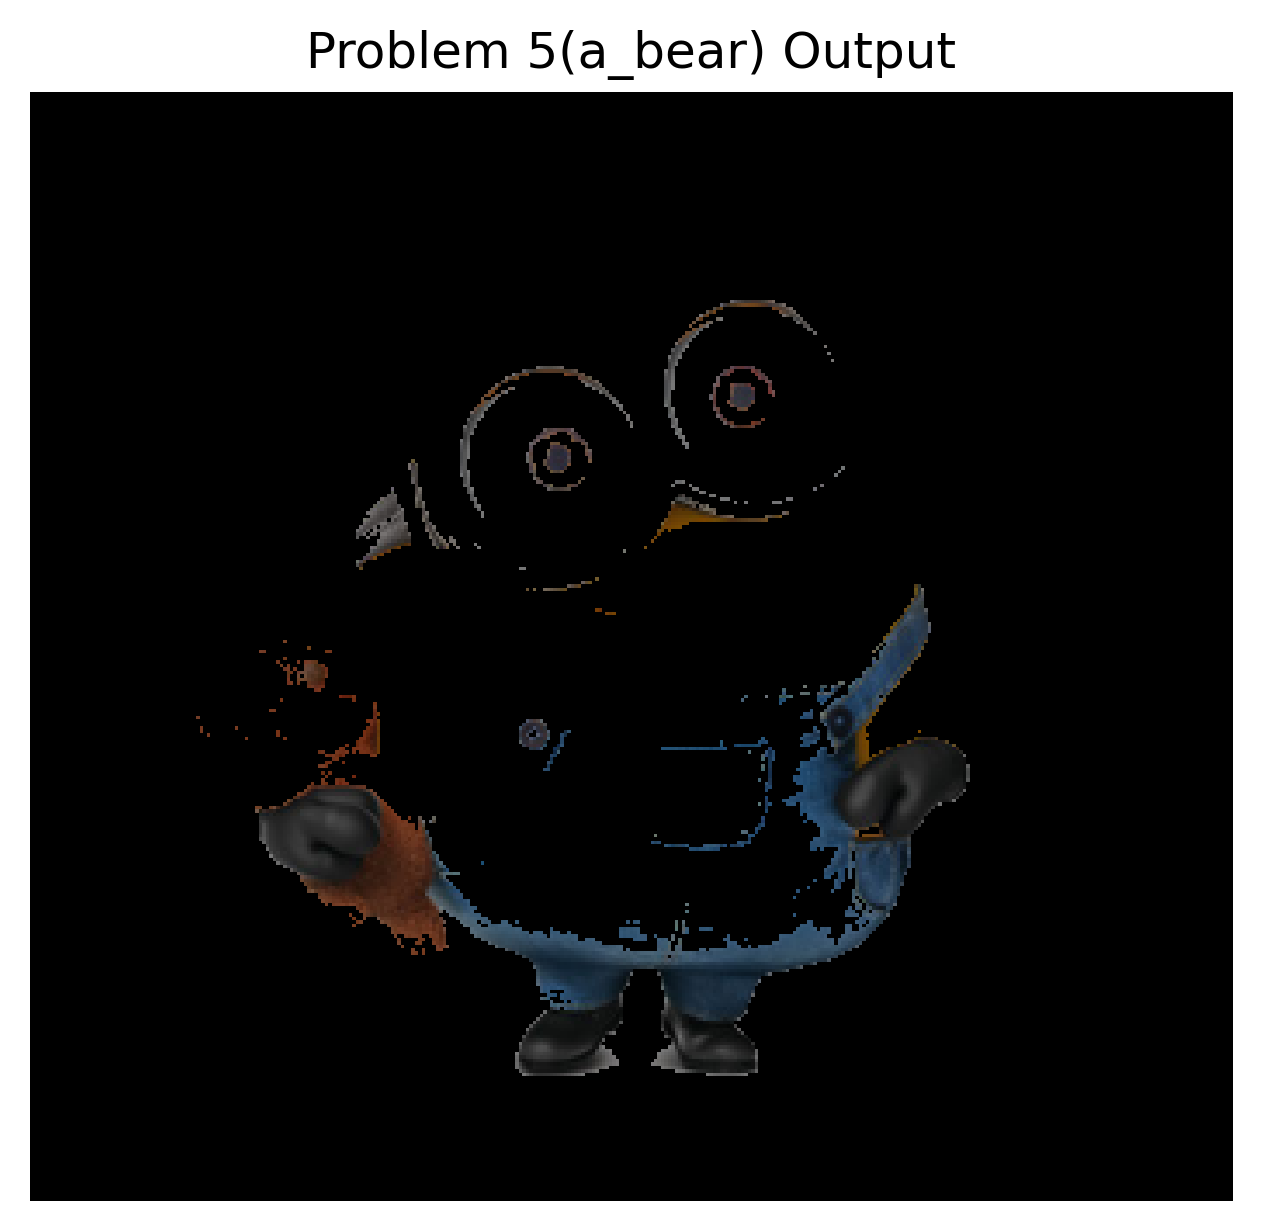
\includegraphics[width=0.45\textwidth]{plots/P5_a_bear_output.png}
	\end{center}
	
	\vspace{0.75em}
	\noindent\textbf{(b) Detect skin color (yellow-like).}
	For the minion’s yellow body (skin-like yellow), the thresholds were adjusted to keep pixels with strong red and green components (yellow is roughly high R and high G) while restricting blue so that the jeans and background are not selected. The resulting detected region area was \textbf{10540 pixels}. The output image mainly preserves the yellow regions of the minion.
	
	\begin{center}
		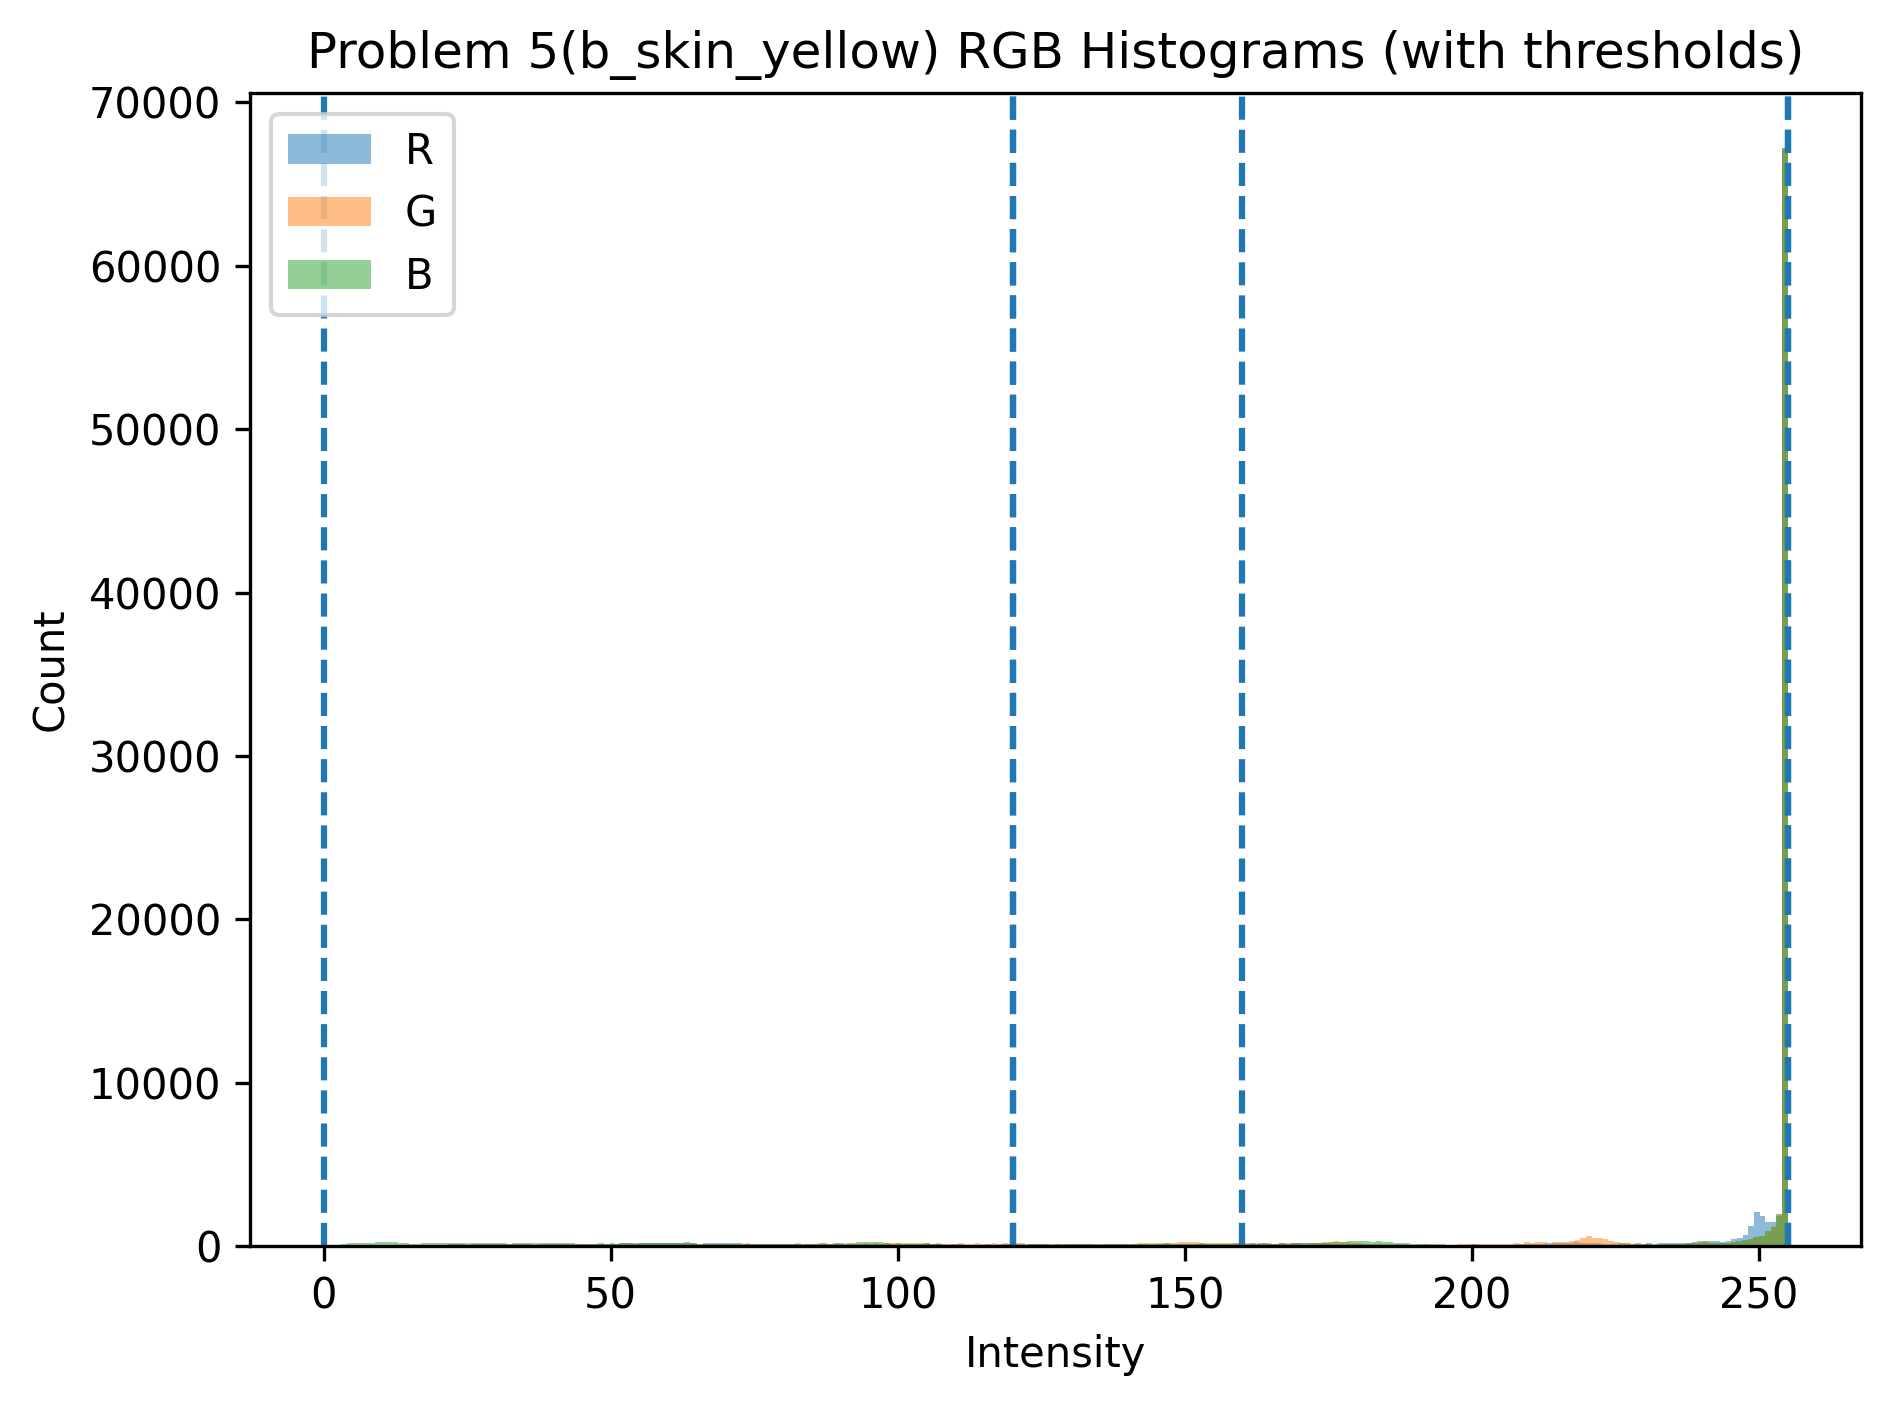
\includegraphics[width=0.45\textwidth]{plots/P5_b_skin_yellow_hist.png}\hfill
		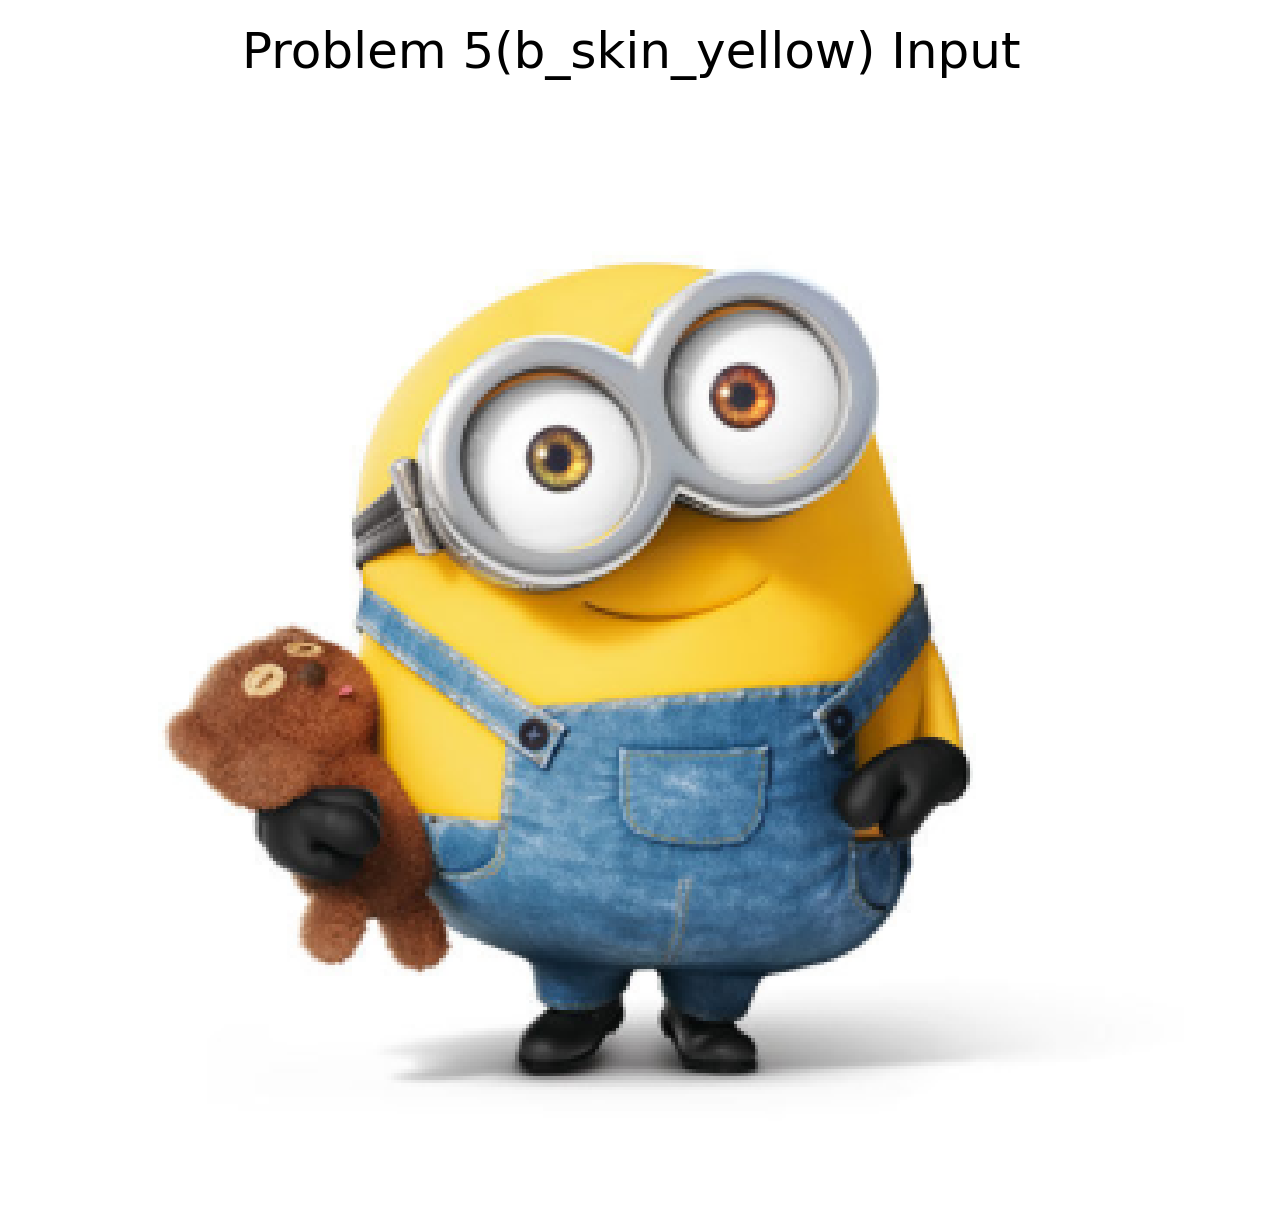
\includegraphics[width=0.45\textwidth]{plots/P5_b_skin_yellow_input.png}\\[0.5em]
		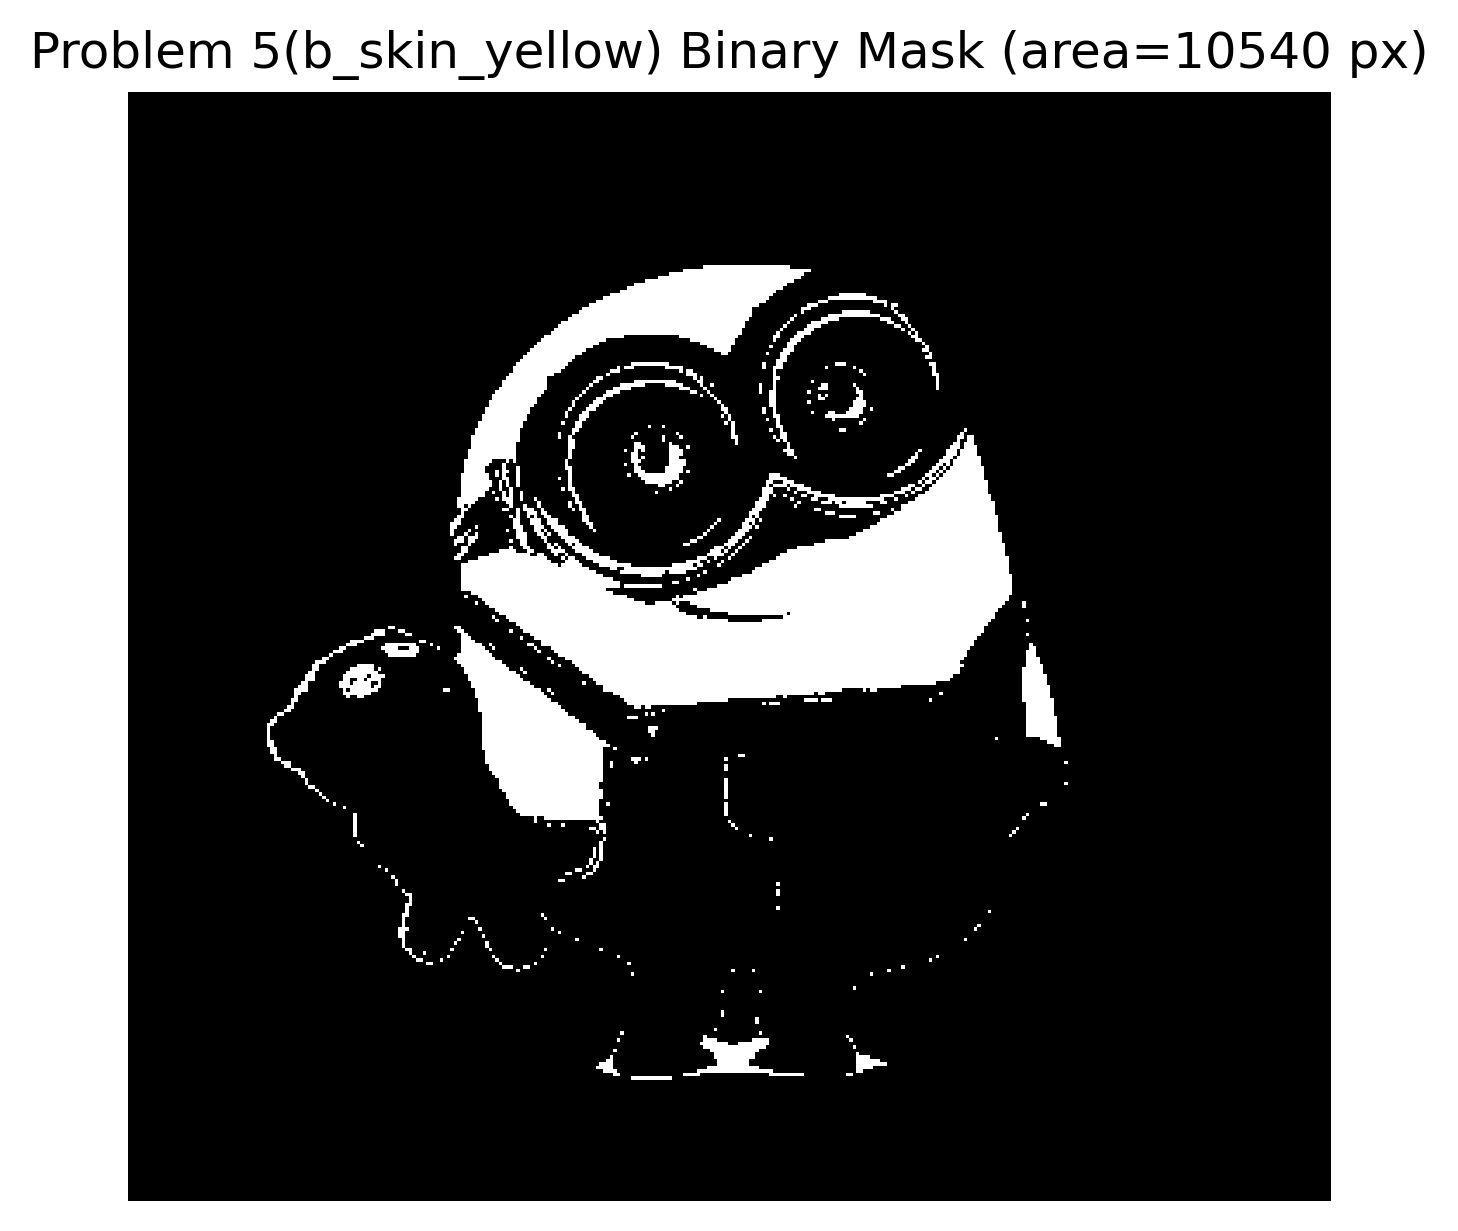
\includegraphics[width=0.45\textwidth]{plots/P5_b_skin_yellow_mask.png}\hfill
		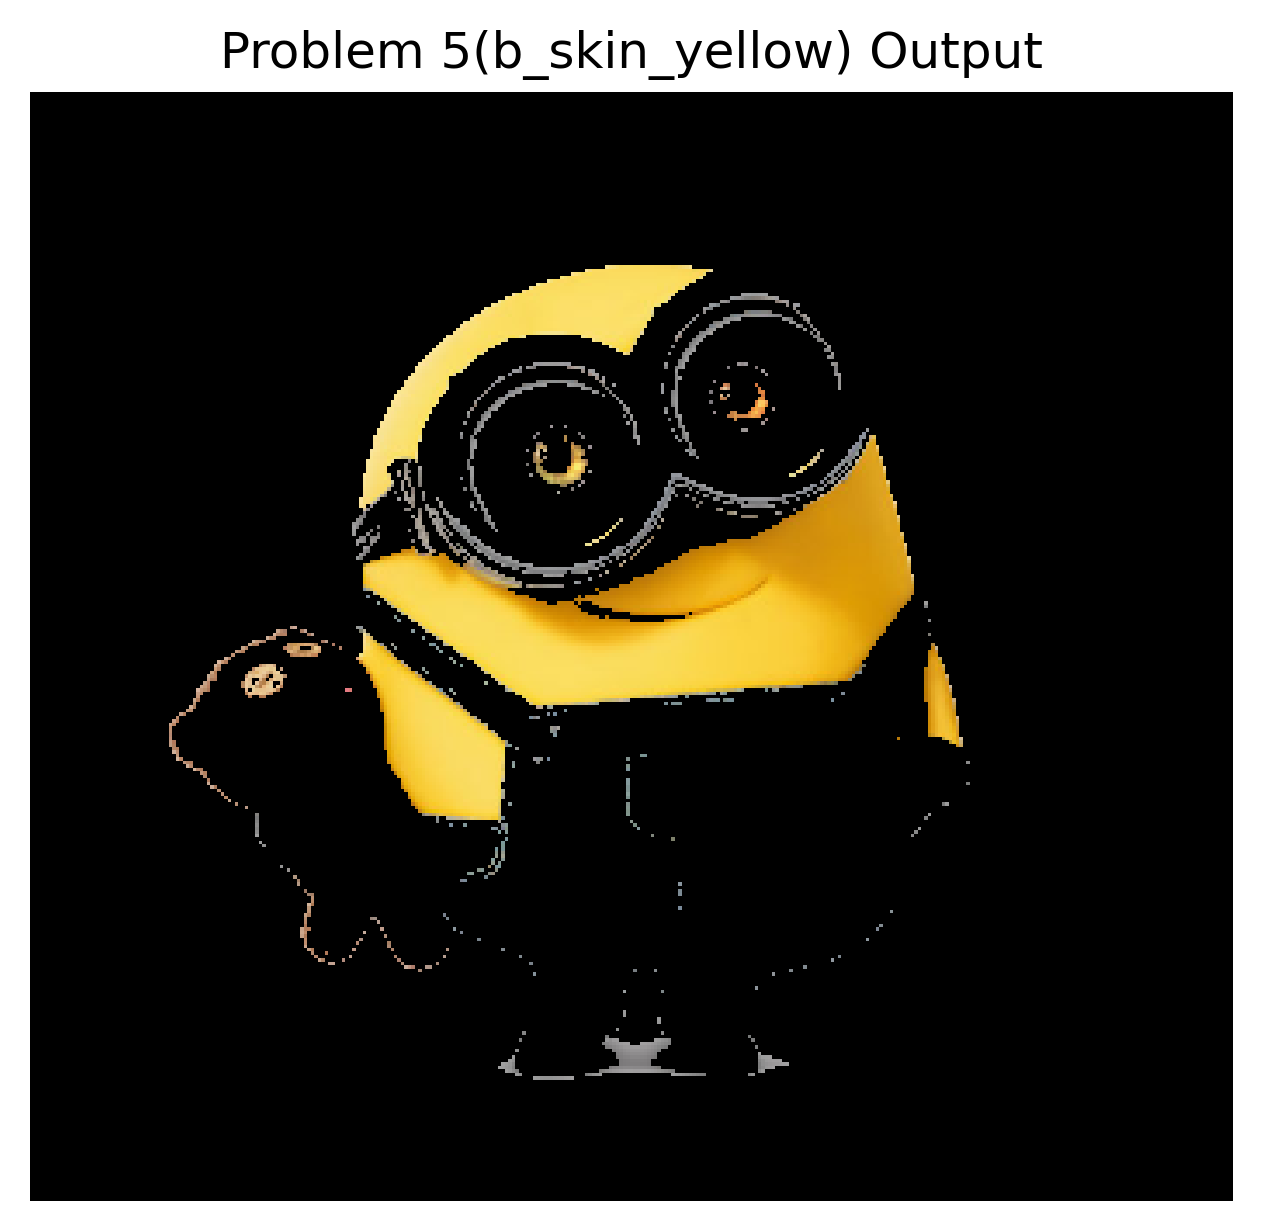
\includegraphics[width=0.45\textwidth]{plots/P5_b_skin_yellow_output.png}
	\end{center}
	
	\vspace{0.75em}
	\noindent\textbf{(c) Detect clothes (blue overalls).}
	For the blue overalls, I selected thresholds that keep pixels with a comparatively stronger blue component and moderate red/green values, which suppresses the yellow body and the background. The resulting detected region area was \textbf{2974 pixels}. The output image highlights the clothing region, though small scattered detections can appear due to shading and reflections.
	
	\begin{center}
		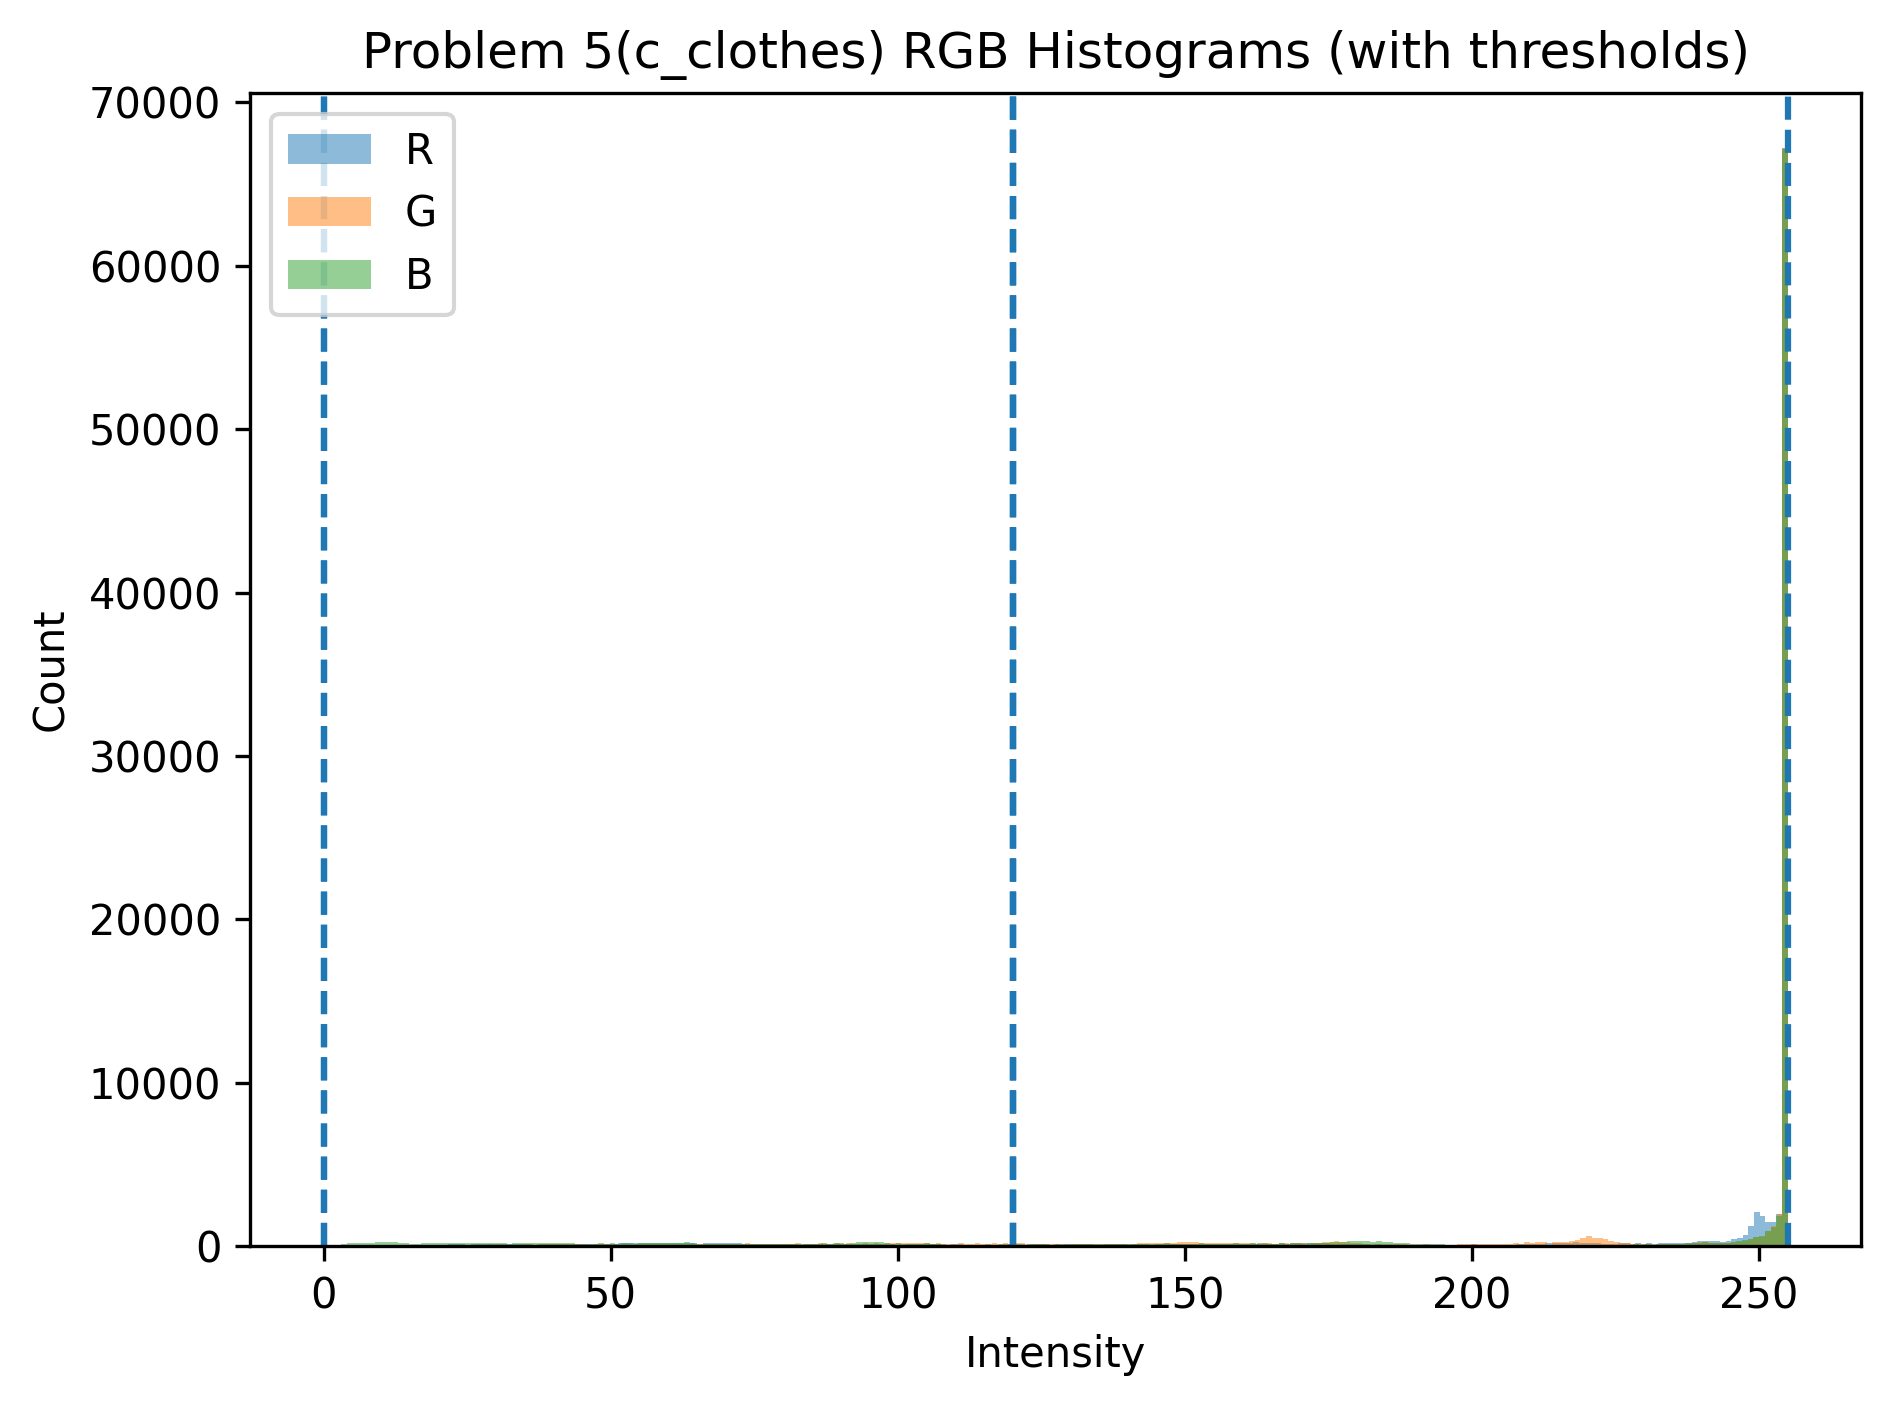
\includegraphics[width=0.45\textwidth]{plots/P5_c_clothes_hist.png}\hfill
		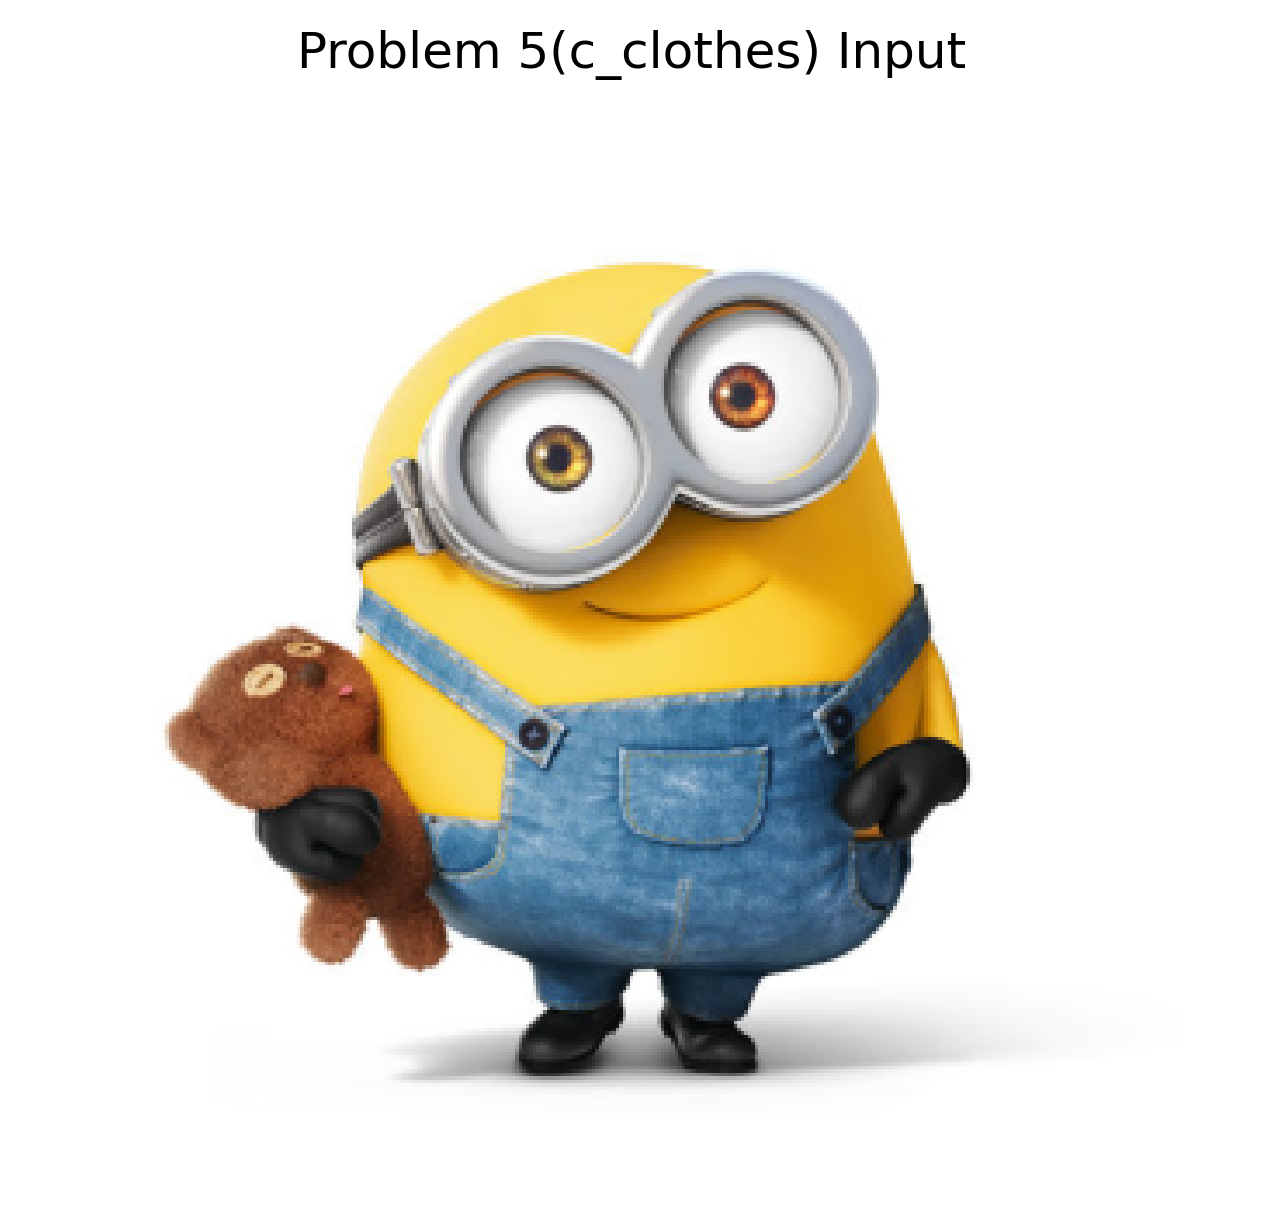
\includegraphics[width=0.45\textwidth]{plots/P5_c_clothes_input.png}\\[0.5em]
		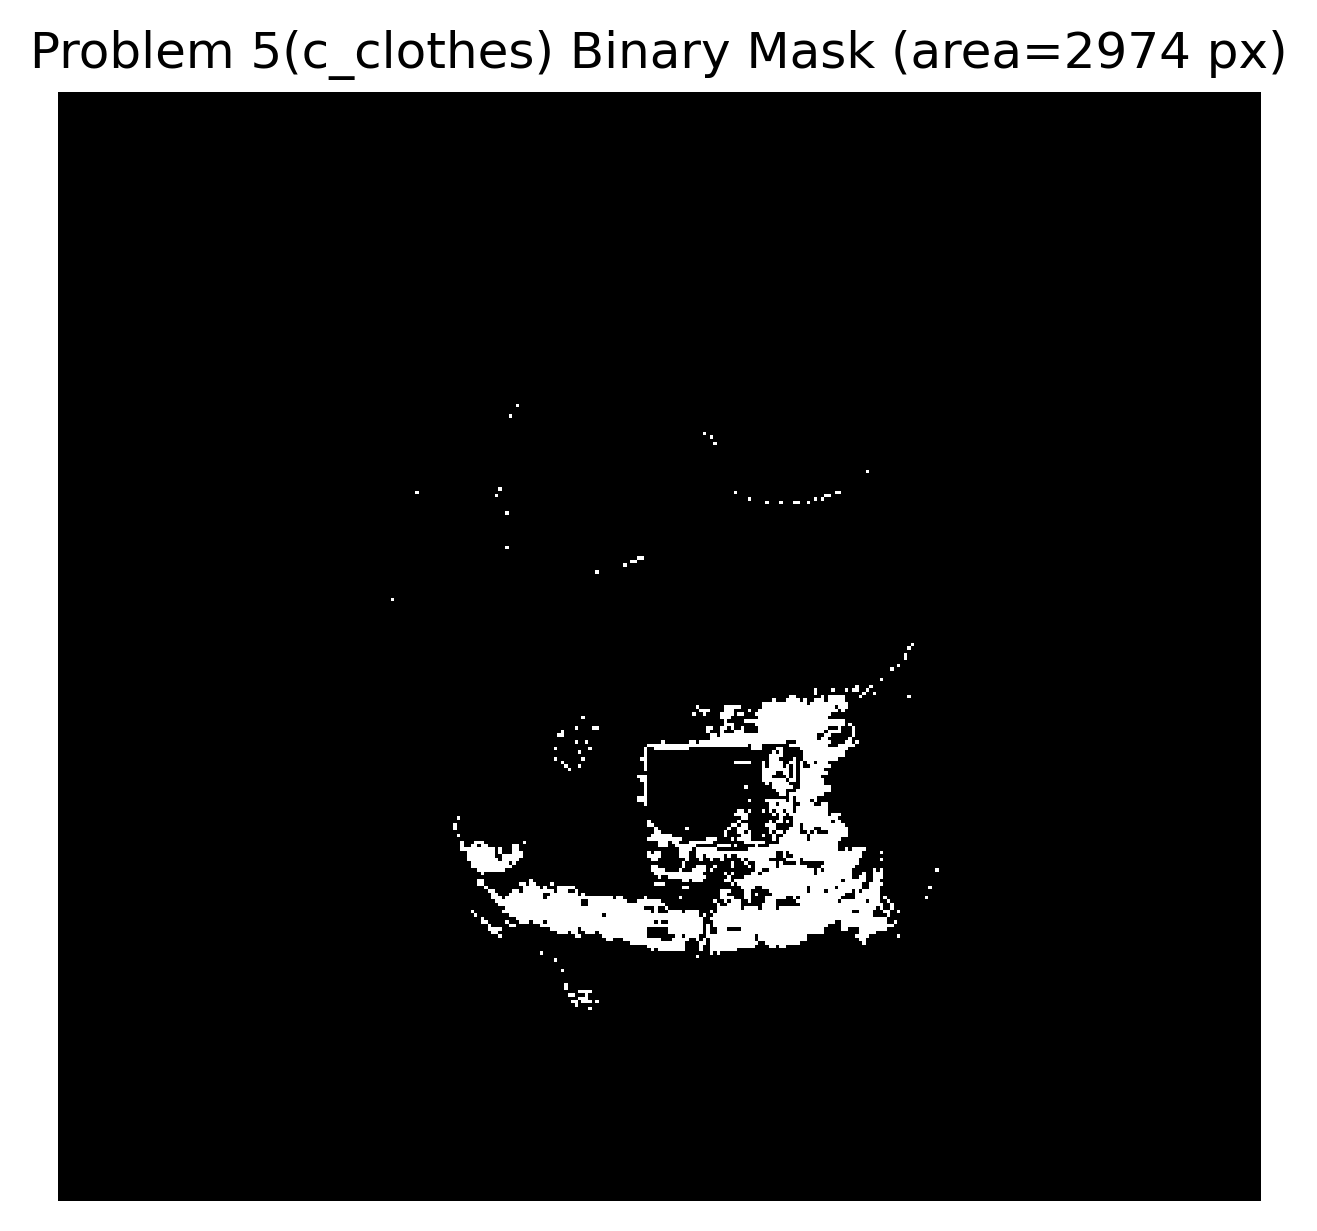
\includegraphics[width=0.45\textwidth]{plots/P5_c_clothes_mask.png}\hfill
		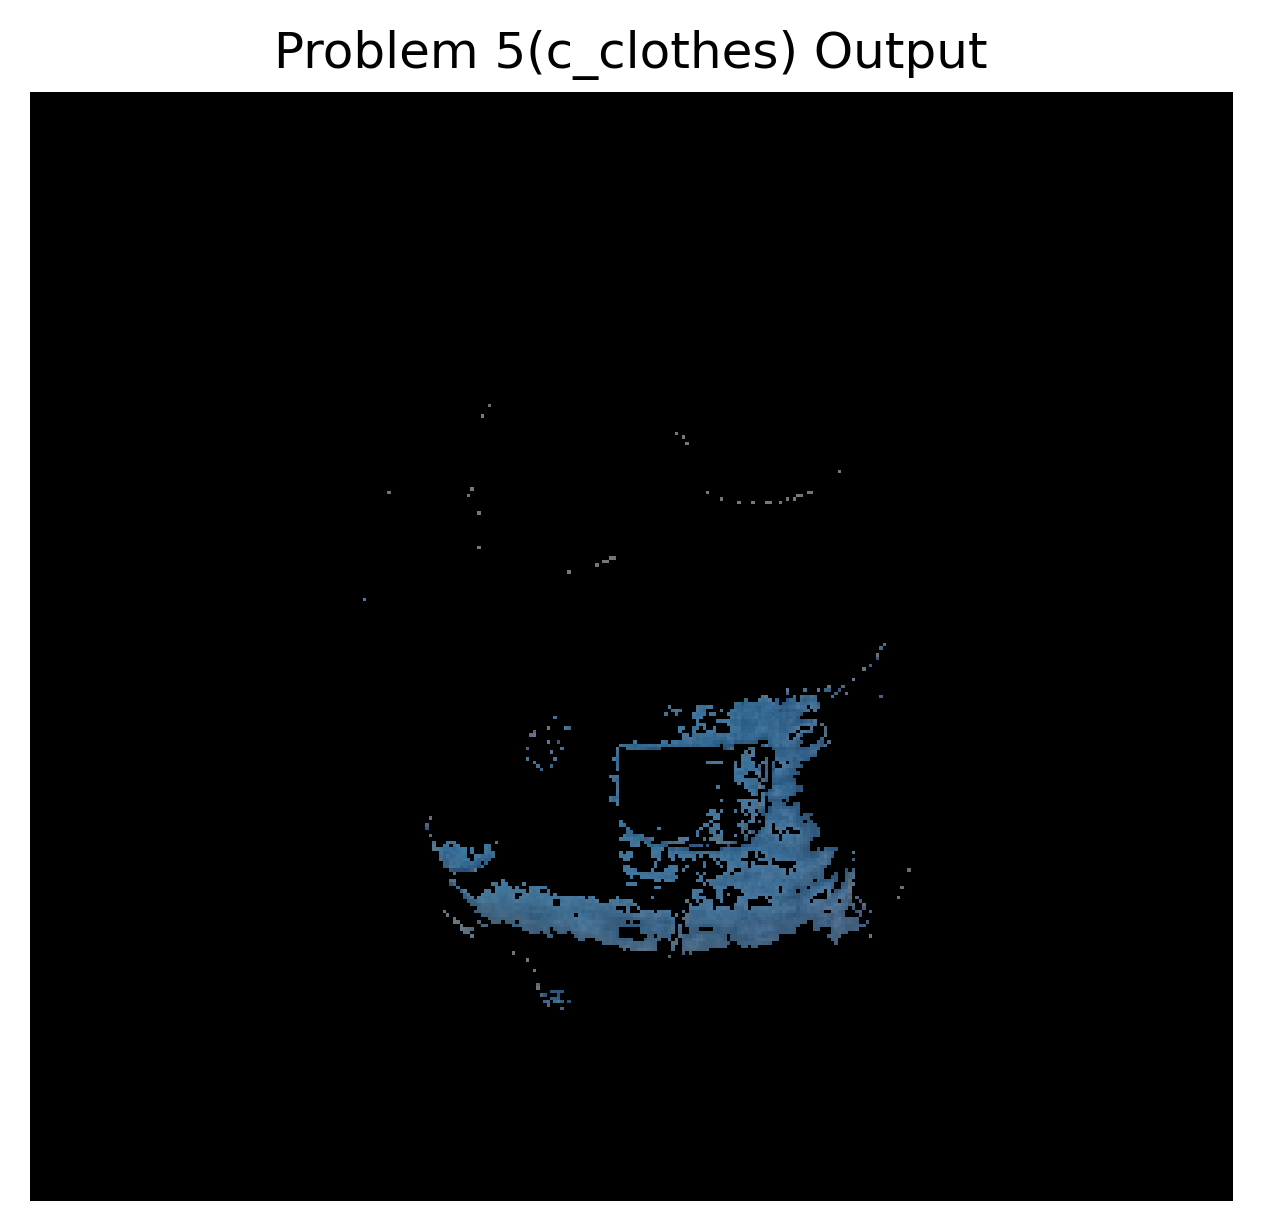
\includegraphics[width=0.45\textwidth]{plots/P5_c_clothes_output.png}
	\end{center}
	
	\vspace{0.5em}
	\noindent\textbf{Discussion.}
	This histogram-based segmentation is simple and fast, but the mask quality depends strongly on lighting and shading. Highlights and shadows shift pixel intensities, which can cause small holes or scattered detections. Nevertheless, by selecting threshold ranges directly from the histogram peaks/tails, I was able to isolate (a) the bear, (b) yellow skin/body, and (c) the blue clothes with reasonable accuracy.
	
	\newpage

	% ---------------- Problem 6 ----------------
	\noindent\textbf{Problem 6. Video Creation (40 points)}
	
	Use the
	\href{https://github.com/pattichis/AIML/blob/main/Session_8_Create_videos.ipynb}{video creation tutorial}
	and
	\href{https://github.com/pattichis/AIML/blob/main/Session_8_Video_template.ipynb}{video template}. Construct a fun video that satisfies the following requirements:
	
	\begin{enumerate}[label=\textbf{(\alph*)}, leftmargin=1.2cm]
		\item Uses NumPy arrays and uses at least 10 frames and a maximum of 30 frames.
		\item You have two small objects moving in the video.
	\end{enumerate}
	
	Submit the final video and a printout of the PDF of the Jupyter notebook that you used to create it.
	
	
	\vspace{1em}
	\noindent\textbf{Solution.}
	
	In appendix below.
	
	\newpage
	
	\begin{lstlisting}
"""
=====================================================
ECE 533 - Homework 1
Scott Nguyen
Problems 1–6
All outputs saved to ./plots
=====================================================
"""

import os
import numpy as np
import cv2
import matplotlib.pyplot as plt
import torch
import torch.nn.functional as F
from AOLME import *
from IPython.display import HTML


# =================================================
# Functions
# =================================================
def ensure_plot_dir():
base = os.path.dirname(__file__)
p = os.path.join(base, "plots")
os.makedirs(p, exist_ok=True)
return p


def save_gray(img, title, filename, vmin=0, vmax=255):
plt.figure()
plt.imshow(img, cmap='gray', vmin=vmin, vmax=vmax)
plt.title(title)
plt.axis('off')
plt.savefig(os.path.join(plot_dir, filename), dpi=300, bbox_inches='tight')
plt.close()


def save_rgb(img, title, filename):
plt.figure()
plt.imshow(img)
plt.title(title)
plt.axis('off')
plt.savefig(os.path.join(plot_dir, filename), dpi=300, bbox_inches='tight')
plt.close()


def log_transform(I, C):
J = np.log1p(C * I.astype(np.float32))
J = (J - J.min()) / (J.max() - J.min()) * 255
return J.astype(np.uint8)


def relu(x):
return np.maximum(0, x)


def sigmoid(x):
return 1 / (1 + np.exp(-x))


def max_pool(I, k, stride=1):
t = torch.from_numpy(I).float()[None, None, :, :]
return F.max_pool2d(t, kernel_size=k, stride=stride).squeeze().numpy()


def erosion(I, k):
t = torch.from_numpy(I).float()[None, None, :, :]
return (-F.max_pool2d(-t, kernel_size=k, stride=1)).squeeze().numpy()


def imread_rgb_resize(path, h=320):
bgr = cv2.imread(path)
H, W = bgr.shape[:2]
bgr = cv2.resize(bgr, (int(W * h / H), h))
return cv2.cvtColor(bgr, cv2.COLOR_BGR2RGB)


def threshold_mask(rgb, r0, r1, g0, g1, b0, b1):
r, g, b = rgb[:,:,0], rgb[:,:,1], rgb[:,:,2]
return ((r>=r0)&(r<=r1)&(g>=g0)&(g<=g1)&(b>=b0)&(b<=b1)).astype(np.uint8)


def apply_mask(rgb, m):
out = rgb.copy()
out[m==0] = 0
return out


# =================================================
plot_dir = ensure_plot_dir()


# =================================================
# Problem 1
# =================================================
binary = np.indices((8,8)).sum(axis=0) % 2
save_gray(binary, "Problem 1(a) Binary", "binary.png", 0, 1)

row = np.linspace(0,255,8,dtype=np.uint8)
gray = np.tile(row,(8,1))
save_gray(gray, "Problem 1(b) Grayscale", "grayscale.png")

color = np.zeros((8,8,3),dtype=np.uint8)
color[:4,:4]=[255,0,0]
color[:4,4:]=[0,255,0]
color[4:,:4]=[0,0,255]
color[4:,4:]=[255,255,0]
save_rgb(color, "Problem 1(c) Color", "color.png")


# =================================================
# Problem 2
# =================================================
A = np.full((128,128),128,np.uint8)
A[48:80,48:80]=129
save_gray(A,"P2(A) Min contrast","P2A.png")

B = np.zeros((128,128),np.uint8)
B[32:96,32:96]=255
save_gray(B,"P2(B) Max contrast","P2B.png")

vals=[5,10,100,200,250]
C = np.zeros((200,400),np.uint8)
for i,v in enumerate(vals):
C[40:160,30+i*80:90+i*80]=v
save_gray(C,"P2(C) Patches","P2C.png")

for c in [1,5,10,100]:
save_gray(log_transform(C,c),f"P2(D) Log C={c}",f"P2D_{c}.png")


# =================================================
# Problem 3
# =================================================
img=np.zeros((150,300),np.uint8)
img[40:120,40:120]=5
img[40:120,180:260]=100
save_gray(img,"P3(a) Original","P3A.png")

rimg = relu(img-20)
rimg=(rimg/rimg.max()*255).astype(np.uint8)
save_gray(rimg,"P3(b) ReLU","P3B.png")

simg=sigmoid(0.1*(img-20))
simg=((simg-simg.min())/(simg.max()-simg.min())*255).astype(np.uint8)
save_gray(simg,"P3(c) Sigmoid","P3C.png")


# =================================================
# Problem 4
# =================================================
I=np.random.randint(0,256,(64,64)).astype(np.float32)
save_gray(I,"P4 Input","P4A.png")

pool=max_pool(I,4,4)
save_gray(pool,"P4 MaxPool","P4B.png")

ero=erosion(I,3)
save_gray(ero,"P4 Erosion","P4C.png")


# =================================================
# Problem 5
# =================================================
rgb=imread_rgb_resize("Bob.jpg")

cases={
	"a_bear":(0,120,0,120,0,120),
	"b_skin":(120,255,120,255,0,160),
	"c_clothes":(0,120,0,120,120,255)
}

for name,t in cases.items():
m=threshold_mask(rgb,*t)
out=apply_mask(rgb,m)
save_rgb(rgb,f"P5 {name} input",f"P5_{name}_input.png")
save_gray(m*255,f"P5 {name} mask",f"P5_{name}_mask.png")
save_rgb(out,f"P5 {name} output",f"P5_{name}_output.png")


# =================================================
# Problem 6
# =================================================
rows,cols=20,20
gray="%02x%02x%02x"%(120,120,120)
orange="%02x%02x%02x"%(255,165,0)
cyan="%02x%02x%02x"%(0,255,255)

frames=[]
r1,c1,dr1,dc1=2,2,1,1
r2,c2,dr2,dc2=14,12,-1,1

for _ in range(20):
f=np.full((rows,cols),gray)
f[r1:r1+2,c1:c1+2]=orange
f[r2:r2+3,c2:c2+3]=cyan
frames.append(f)

r1+=dr1; c1+=dc1
r2+=dr2; c2+=dc2

if r1<=0 or r1>=rows-2: dr1*=-1
if c1<=0 or c1>=cols-2: dc1*=-1
if r2<=0 or r2>=rows-3: dr2*=-1
if c2<=0 or c2>=cols-3: dc2*=-1

play_video = vid_show(frames, 10)
play_video.save(os.path.join(plot_dir, "problem6_video.mp4"))
	\end{lstlisting}
\end{document}
